% Options for packages loaded elsewhere
\PassOptionsToPackage{unicode}{hyperref}
\PassOptionsToPackage{hyphens}{url}
\PassOptionsToPackage{dvipsnames,svgnames,x11names}{xcolor}
%
\documentclass[
  10pt,
]{article}

\usepackage{amsmath,amssymb}
\usepackage{iftex}
\ifPDFTeX
  \usepackage[T1]{fontenc}
  \usepackage[utf8]{inputenc}
  \usepackage{textcomp} % provide euro and other symbols
\else % if luatex or xetex
  \usepackage{unicode-math}
  \defaultfontfeatures{Scale=MatchLowercase}
  \defaultfontfeatures[\rmfamily]{Ligatures=TeX,Scale=1}
\fi
\usepackage{lmodern}
\ifPDFTeX\else  
    % xetex/luatex font selection
    \setmainfont[]{Helvetica}
    \setmonofont[]{Roboto}
\fi
% Use upquote if available, for straight quotes in verbatim environments
\IfFileExists{upquote.sty}{\usepackage{upquote}}{}
\IfFileExists{microtype.sty}{% use microtype if available
  \usepackage[]{microtype}
  \UseMicrotypeSet[protrusion]{basicmath} % disable protrusion for tt fonts
}{}
\makeatletter
\@ifundefined{KOMAClassName}{% if non-KOMA class
  \IfFileExists{parskip.sty}{%
    \usepackage{parskip}
  }{% else
    \setlength{\parindent}{0pt}
    \setlength{\parskip}{6pt plus 2pt minus 1pt}}
}{% if KOMA class
  \KOMAoptions{parskip=half}}
\makeatother
\usepackage{xcolor}
\setlength{\emergencystretch}{3em} % prevent overfull lines
\setcounter{secnumdepth}{2}
% Make \paragraph and \subparagraph free-standing
\makeatletter
\ifx\paragraph\undefined\else
  \let\oldparagraph\paragraph
  \renewcommand{\paragraph}{
    \@ifstar
      \xxxParagraphStar
      \xxxParagraphNoStar
  }
  \newcommand{\xxxParagraphStar}[1]{\oldparagraph*{#1}\mbox{}}
  \newcommand{\xxxParagraphNoStar}[1]{\oldparagraph{#1}\mbox{}}
\fi
\ifx\subparagraph\undefined\else
  \let\oldsubparagraph\subparagraph
  \renewcommand{\subparagraph}{
    \@ifstar
      \xxxSubParagraphStar
      \xxxSubParagraphNoStar
  }
  \newcommand{\xxxSubParagraphStar}[1]{\oldsubparagraph*{#1}\mbox{}}
  \newcommand{\xxxSubParagraphNoStar}[1]{\oldsubparagraph{#1}\mbox{}}
\fi
\makeatother


\providecommand{\tightlist}{%
  \setlength{\itemsep}{0pt}\setlength{\parskip}{0pt}}\usepackage{longtable,booktabs,array}
\usepackage{calc} % for calculating minipage widths
% Correct order of tables after \paragraph or \subparagraph
\usepackage{etoolbox}
\makeatletter
\patchcmd\longtable{\par}{\if@noskipsec\mbox{}\fi\par}{}{}
\makeatother
% Allow footnotes in longtable head/foot
\IfFileExists{footnotehyper.sty}{\usepackage{footnotehyper}}{\usepackage{footnote}}
\makesavenoteenv{longtable}
\usepackage{graphicx}
\makeatletter
\newsavebox\pandoc@box
\newcommand*\pandocbounded[1]{% scales image to fit in text height/width
  \sbox\pandoc@box{#1}%
  \Gscale@div\@tempa{\textheight}{\dimexpr\ht\pandoc@box+\dp\pandoc@box\relax}%
  \Gscale@div\@tempb{\linewidth}{\wd\pandoc@box}%
  \ifdim\@tempb\p@<\@tempa\p@\let\@tempa\@tempb\fi% select the smaller of both
  \ifdim\@tempa\p@<\p@\scalebox{\@tempa}{\usebox\pandoc@box}%
  \else\usebox{\pandoc@box}%
  \fi%
}
% Set default figure placement to htbp
\def\fps@figure{htbp}
\makeatother
% definitions for citeproc citations
\NewDocumentCommand\citeproctext{}{}
\NewDocumentCommand\citeproc{mm}{%
  \begingroup\def\citeproctext{#2}\cite{#1}\endgroup}
\makeatletter
 % allow citations to break across lines
 \let\@cite@ofmt\@firstofone
 % avoid brackets around text for \cite:
 \def\@biblabel#1{}
 \def\@cite#1#2{{#1\if@tempswa , #2\fi}}
\makeatother
\newlength{\cslhangindent}
\setlength{\cslhangindent}{1.5em}
\newlength{\csllabelwidth}
\setlength{\csllabelwidth}{3em}
\newenvironment{CSLReferences}[2] % #1 hanging-indent, #2 entry-spacing
 {\begin{list}{}{%
  \setlength{\itemindent}{0pt}
  \setlength{\leftmargin}{0pt}
  \setlength{\parsep}{0pt}
  % turn on hanging indent if param 1 is 1
  \ifodd #1
   \setlength{\leftmargin}{\cslhangindent}
   \setlength{\itemindent}{-1\cslhangindent}
  \fi
  % set entry spacing
  \setlength{\itemsep}{#2\baselineskip}}}
 {\end{list}}
\usepackage{calc}
\newcommand{\CSLBlock}[1]{\hfill\break\parbox[t]{\linewidth}{\strut\ignorespaces#1\strut}}
\newcommand{\CSLLeftMargin}[1]{\parbox[t]{\csllabelwidth}{\strut#1\strut}}
\newcommand{\CSLRightInline}[1]{\parbox[t]{\linewidth - \csllabelwidth}{\strut#1\strut}}
\newcommand{\CSLIndent}[1]{\hspace{\cslhangindent}#1}

\usepackage{orcidlink}
\definecolor{mypink}{RGB}{219, 48, 122}
\usepackage[dvipsnames]{xcolor} % colors
\renewcommand{\thefootnote}{\arabic{footnote}}
\newcommand{\ear}[1]{{\textcolor{blue}{#1}}}
\newcommand{\svp}[1]{{\textcolor{RedOrange}{#1}}}
\newcommand{\hh}[1]{{\textcolor{Green}{#1}}}
\makeatletter
\@ifpackageloaded{caption}{}{\usepackage{caption}}
\AtBeginDocument{%
\ifdefined\contentsname
  \renewcommand*\contentsname{Table of contents}
\else
  \newcommand\contentsname{Table of contents}
\fi
\ifdefined\listfigurename
  \renewcommand*\listfigurename{List of Figures}
\else
  \newcommand\listfigurename{List of Figures}
\fi
\ifdefined\listtablename
  \renewcommand*\listtablename{List of Tables}
\else
  \newcommand\listtablename{List of Tables}
\fi
\ifdefined\figurename
  \renewcommand*\figurename{Figure}
\else
  \newcommand\figurename{Figure}
\fi
\ifdefined\tablename
  \renewcommand*\tablename{Table}
\else
  \newcommand\tablename{Table}
\fi
}
\@ifpackageloaded{float}{}{\usepackage{float}}
\floatstyle{ruled}
\@ifundefined{c@chapter}{\newfloat{codelisting}{h}{lop}}{\newfloat{codelisting}{h}{lop}[chapter]}
\floatname{codelisting}{Listing}
\newcommand*\listoflistings{\listof{codelisting}{List of Listings}}
\makeatother
\makeatletter
\makeatother
\makeatletter
\@ifpackageloaded{caption}{}{\usepackage{caption}}
\@ifpackageloaded{subcaption}{}{\usepackage{subcaption}}
\makeatother

\usepackage{bookmark}

\IfFileExists{xurl.sty}{\usepackage{xurl}}{} % add URL line breaks if available
\urlstyle{same} % disable monospaced font for URLs
\hypersetup{
  pdftitle={A Guide to Designing Experiments to Test Statistical Graphics},
  colorlinks=true,
  linkcolor={blue},
  filecolor={Maroon},
  citecolor={Blue},
  urlcolor={red},
  pdfcreator={LaTeX via pandoc}}



\title{A Guide to Designing Experiments to Test Statistical
Graphics\thanks{The author(s) received no specific funding for this
work.}}

%% Author information
\author{%
%
Emily Robinson%\footnote{Email: erobin17@calpoly.edu}
~\orcidlink{0000-0001-9800-7304}%
%
\\{\footnotesize Statistics Department}, {\footnotesize California
Polytechnic State University}\\%
Heike Hofmann%\footnote{Email: hhofmann4@unl.edu}
~\orcidlink{0000-0001-6216-5183}%
%
\\{\footnotesize Statistics Department}, {\footnotesize University of
Nebraska - Lincoln}\\%
Susan Vanderplas%\footnote{Email: svanderplas2@unl.edu}
~\orcidlink{0000-0002-3803-0972}%
\footnote{Corresponding author: Susan Vanderplas, svanderplas2@unl.edu}%
\\{\footnotesize Statistics Department}, {\footnotesize University of
Nebraska - Lincoln}\\
}
\begin{document}
\maketitle
\begin{abstract}
In this paper, we discuss considerations and methods for experimentally
testing visualizations. We discuss levels of user engagement with
graphics, common issues when developing a sampling or data generation
model, the importance of pilot testing, and data analysis methods. Along
the way, we also provide recommendations of how to avoid some of the
unique pitfalls of human testing in statistical and visualization
research.
\end{abstract}


\section{Introduction}\label{introduction}

Data visualizations are a critically important tool for communicating
scientific information to the public in what creators hope is an
easy-to-digest, visually attractive form. There are many strategies for
creating charts and graphs, from Tufte-esque minimalism (Tufte, 1991) to
charts designed with extra imagery and aesthetic appeal that draw the
viewer's attention and persist in memory (Cairo, 2012). For a specific
type of data, there are also usually many different chart forms to
display that data: for instance, if we have a set of categorical data
and we wish to show the relative proportions of each category, we could
do so using a stacked bar chart or the polar equivalent, a pie chart.
There have been several attempts to list out all of the types of charts
(Ribecca, 2022), create a taxonomy of charts (Bertin \& Berg, 1983;
Desnoyers, 2011), and even to create charts using a domain-specific
grammar of graphics (Wilkinson, 1999) that is also useful for
classification. One extremely useful reference is from Data to Viz
(https://www.data-to-viz.com/), which uses a decision tree to show
different visualizations compatible with the data; R, python, D3.js, and
React code are provided to demonstrate how to create those
visualizations. With all of the different design choices available, how
are chart creators to know what is the best approach for communicating
data to the appropriate audience?

While there are heuristics, general guidelines, and best practices
(Allen \& Erhardt, 2016; Few, 2006; Haemer, 1948; Kosslyn, 2006;
presentation, 1915) for creating useful and visually attractive data
displays, the best way to establish the efficacy of various design
decisions is to test the visualization on humans, evaluating different
variants under controlled conditions (Cleveland et al., 1988; Cleveland
\& McGill, 1985). Empirical assessments of visualizations, when
carefully designed, allow statisticians to determine which
representation of the same data is most effective along one or more
dimension(s) of interest: estimation or prediction accuracy, within or
between group comparisons, response time, and ability to draw real-world
decisions are common goals for charts.

It is extremely challenging to design studies which strike the right
balance between experimental control (i.e.~internal validity) and
generalizability to a wider context (i.e.~external validity). Simply
asking people to read quantities off of a graph may not generalize
beyond the questions asked or the data used in the chart (Croxton, 1932;
Croxton \& Stryker, 1927; Eells, 1926; Huhn, 1927), but designing a
study that is sufficiently robust to those issues requires manipulation
or control of so many factors that the amount of participants and trials
quickly becomes daunting or unaffordable. In addition, when conducting
graphics experiments, researchers are in the unusual position of being
both the subject matter expert and the statistician, providing an
unusual amount of control over not just the experimental design but also
the specific treatments, levels, and experimental protocols. The amount
of choices required to develop, pilot, and run an experiment can be
overwhelming. In this paper, we attempt to distill the experience gained
from conducting several different types of graphics experiments (Hofmann
et al., 2012; Robinson, 2022; Vanderplas et al., 2019, 2024; Vanderplas
\& Hofmann, 2015, 2017), discussing the use of different testing methods
(Vanderplas et al., 2020), the process of designing a graphical
experiment, and analysis of the resulting empirical data. It is our hope
that this paper will lower the barriers that exist for conducting
empirical graphics research and reduce the probability of costly
mistakes.

Section~\ref{sec-testing-methods} discusses different methods for
testing graphics, and which methods best address different levels of
user engagement. In Section~\ref{sec-model-dev}, we discuss the process
of developing the data-generating model used to control the statistical
features of data in the tested visualizations. Model development is a
nuanced and iterative process that ultimately determines the success and
generalizability of the experimental results. In
Section~\ref{sec-exp-dev}, we discuss the design of the experimental
protocol - the choice of platform, number and type of trials, and flow
of the experiment. We briefly consider different experimental design
considerations in Section~\ref{sec-exp-design}, but focus primarily on
factors specific to graphics experiments, and then move to the
importance of pilot testing in Section~\ref{sec-pilot-test}. Finally, we
provide some common analysis strategies in Section~\ref{sec-analysis},
including strategies for handling the unexpected data features which are
so common in graphical testing experiments.

\section{Testing Methods and User Engagement}\label{sec-testing-methods}

There are many different testing methods used to empirically assess
statistical graphics. This paper uses studies conducted online without
additional equipment as primary examples, though many of the same
considerations apply to in-person experiments conducted using additional
equipment, including 3D printed charts, eye-tracking equipment, and
interactive data displays. Online experiments have lower overhead, offer
relatively fast data collection, and provide useful results for
well-designed experiments. The toolkit used for these experiments is
R-based (R Core Team, 2022), and includes ggplot2 (Wickham, 2016) and
Shiny (Chang et al., 2021) as primary components. In many experiments,
we customized the Shiny interface with JavaScript and D3 (Bostock et
al., 2011), enabling interactive graphics, use of svgs, and other useful
extensions. While we prefer this set of tools, most of the observations
described here apply to a wide variety of different workflows for
graphical experimentation, including in-person experiments.

It is important to consider the level of user engagement which is
necessary to complete a particular visual or graphical task. For
instance, testing whether someone can detect an effect such as a linear
trend in noisy data is a perceptual question. Perceptual questions are
often examined experimentally using methods which allow the user to
interact with the data on a basic visual level: users are presented with
a visual stimulus and answer yes/no questions to indicate whether the
effect is detected. Numerical estimation is another common task when
testing graphics: in these experiments, the participant views a chart,
estimates the requested numerical quantity, and enters the estimate into
the application through a numerical input, slider, or other form
element. Sometimes, it is possible to set up a scenario where the user
adjusts the plot using a set of controls designed to provide a fixed set
of interactive operations. This type of user engagement was used to
assess the strength of the sine illusion (Vanderplas \& Hofmann, 2015):
users adjusted the strength of a transformation designed to correct the
illusion until the lines appeared to be the same length, as shown in
Figure~\ref{fig-sine-illusion}, providing a direct measure of the
magnitude of the sine illusion's effect. In other situations, it may be
preferable to have the user directly interact with the visual stimulus.
In Vanderplas et al. (2024), participants were asked to rotate and
interact with a 3D rendered bar chart; the application recorded user
interactions and corresponding rotation matrices, providing insight into
the visual comparisons the user may have been performing. This
information was used as a supplement to the explicitly provided
estimates, providing some contextual information as well as the ability
to identify the level of participant engagement with the questions. When
experiments are conducted as part of classroom experiential learning, it
is sometimes helpful to be able to separate the low-effort participants
from those who were fully intellectually engaged in the task.
Interactive graphics provide another level of user engagement that can
be much more open-ended. With interactive graphics, researchers can ask
participants to directly annotate plots, toggle aesthetics, and
highlight groups and plot features. Careful implementation of the
experiment application may allow for each of these interactions to be
recorded and analyzed, producing a rich, if messy, set of data that may
allow researchers to tease apart visual estimation error from common
shortcuts such as rounding used during direct numerical estimation.

\begin{figure}

\centering{

\pandocbounded{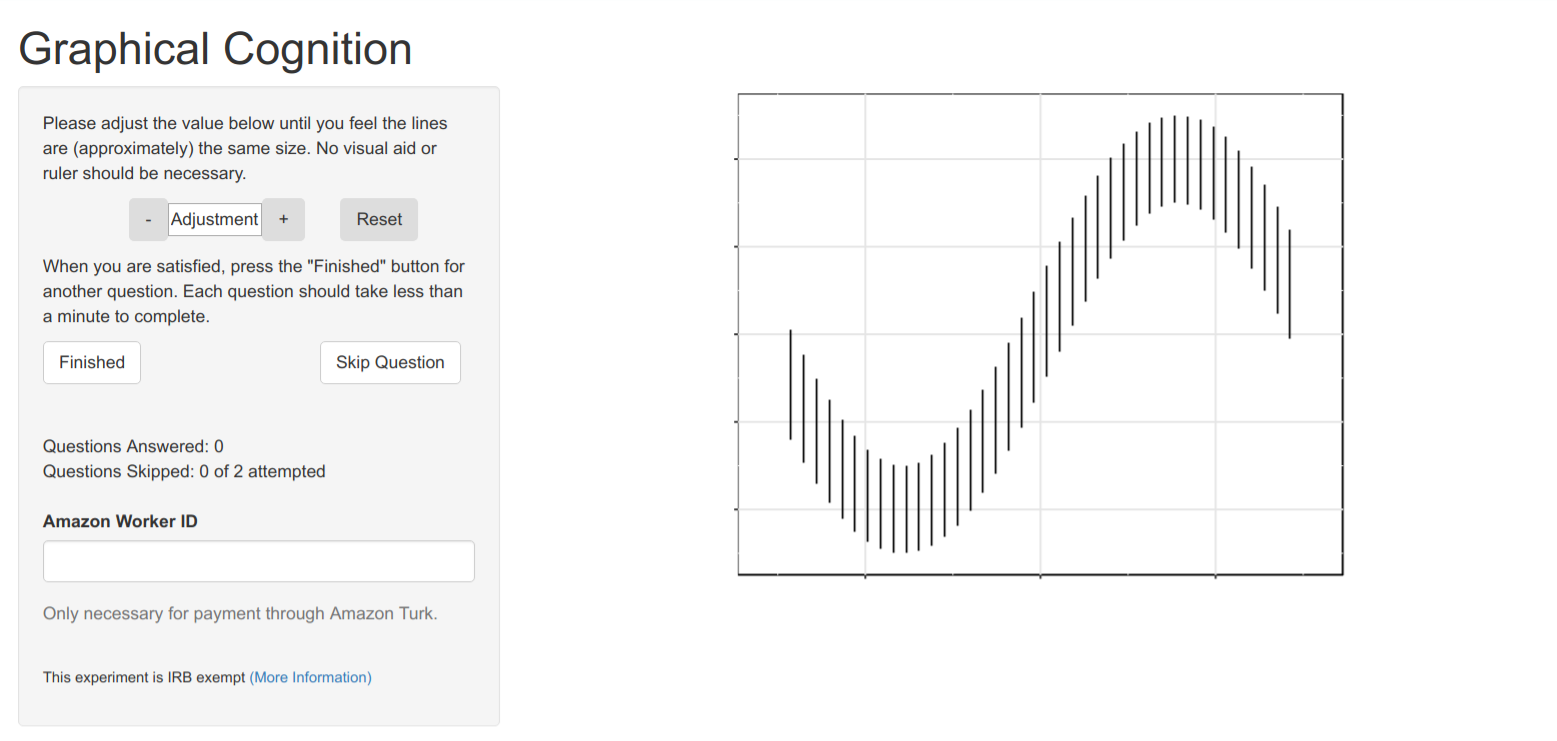
\includegraphics[keepaspectratio]{images/sine_illusion_screenshot.png}}

}

\caption{\label{fig-sine-illusion}Direct adjustment of a plot in a
perceptual task. In this experiment, designed to assess the strength of
the sine illusion, the user adjusts the plot using - and + buttons,
which control the strength of a transformation designed to correct the
effect of the sine illusion. When the user is satisfied that the lines
are of equal length, they select the `Finished' button to move to the
next task. The experiment used a psychophysics experimental design, the
method of adjustment, but leveraged the interactive Shiny interface to
record the entire sequence of adjustments made by the user for each
trial. A demo version of this application can be found at
https://shiny.srvanderplas.com/sine-illusion/.}

\end{figure}%

Visual inference (Buja et al., 2009; Wickham et al., 2010) is another
useful testing tool for perceptual questions such as ``which chart
displays this data more clearly'' (Hofmann et al., 2012) while
simultaneously assessing the statistical significance of the graphical
finding in a chart. Visual inference charts are often called ``lineups''
in analogy to the criminal procedure where the suspect is placed in a
line with several other individuals with similar characteristics. In a
graphical lineup procedure, there is a target plot containing the real
data, embedded in an array of (typically) 19 innocent ``null'' plots
generated through resampling or simulation, for a total of 20 panels. If
viewers consistently pick the target plot at a higher rate than any of
the null plots, the target plot is said to be visually significant (Loy
\& Hofmann, 2013; Majumder et al., 2013) and a ``see'' value, the visual
analogue of a \(p\)-value (Chowdhury et al., 2020), can be calculated
using the \texttt{vinference} R package or the process described in
Vanderplas et al. (2021). The details of this calculation are beyond the
scope of this broader discussion of how to test charts, but more detail
on visual inference is provided in \textless insert citation to visual
inference WIRE article under development\textgreater.

In another variation of the statistical lineup procedure, data generated
from two models are compared, with target plots from each model embedded
in the array of \(K\) total plots. The \(K-2\) null plots are
constructed from a mixture model that blends the two competing models
(Vanderplas \& Hofmann, 2017). Viewers are asked to select the panel(s)
which are most different, and the primary source of information are
trials in which viewers selected the target from one model but not the
other, indicating that the display method used allowed viewers to
differentiate one model's data (but not the other) from the nulls
created through a mixture model. This variation allows the experimenter
to assess graphical design choices to determine whether they effectively
emphasize structural differences in the data (Vanderplas \& Hofmann,
2017).

One advantage of the visual inference technique is that the experimenter
can ask a very general question, such as ``which of these plots is the
most different?'', rather than a specific question about the displayed
data which may require more quantitative sophistication. All of the
necessary information to make the decision is embedded in the choice of
the model used to generate the null plots. This feature is extremely
convenient when conducting the experiment and even allows small children
to complete the task. The downside is that as a result, visual inference
experiments do not allow experimenters to assess the viewer's
understanding of the information shown in the chart. In most cases,
visual inference experiments remove any contextual information from the
charts, including axis labels and values, plot titles, and so on, in
order to encourage participants to make decisions based solely on the
graphical presentation. This lack of context is a double-edged sword:
visual inference can involve participants who do not have any
mathematical training or instincts (including children), but researchers
also cannot use this technique to assess higher levels of engagement
with a chart, such as estimation, prediction, or reasoning based on
displayed information.\\

To assess the viewer's \emph{understanding} of information shown in a
chart, we must ask questions and allow the user to provide feedback.
User feedback may be collected on a numerical scale or through the use
of written comments, recorded ``think-aloud'' processes, and other more
qualitative interaction methods. In some studies, asking users to
interpret a chart within a larger scenario can be effective, as in
Figure~\ref{fig-estimation-describe}, while in others it is more helpful
to ask users to explain answers. In visual inference studies, asking
users why a specific panel was chosen has been demonstrated to provide
rich insight into otherwise confusing numerical results (Vanderplas \&
Hofmann, 2017).

Think-aloud methods ask the viewer to narrate their internal thought
process, either during or after completing a task (Haak et al., 2003).
These recordings (or transcripts) can provide valuable insights into
conscious cognition, and are often used when conducting usability
studies. While we have not to date recorded users talking out loud about
what they are seeing during a study, think aloud methods could easily be
implemented within a Shiny application, with audio recordings saved to
the server for transcription and analysis (Dunbar, 1995; Kirschenbaum,
2003; Trafton et al., 2000). It is even possible that these recordings
could be automatically transcribed using speech-to-text models. We have
used think-aloud methods informally during pilot studies to ``harden''
graphical experiments and verify the selection of parameters used in an
experiment. The success of this approach, combined with the few studies
which used think-aloud to assess charts (Haider et al., 2021; Kulhavy et
al., 1992; Lee et al., 2016), suggests that think-aloud methods are an
often-overlooked but useful tool for assessing data visualizations.

\begin{figure}

\centering{

\pandocbounded{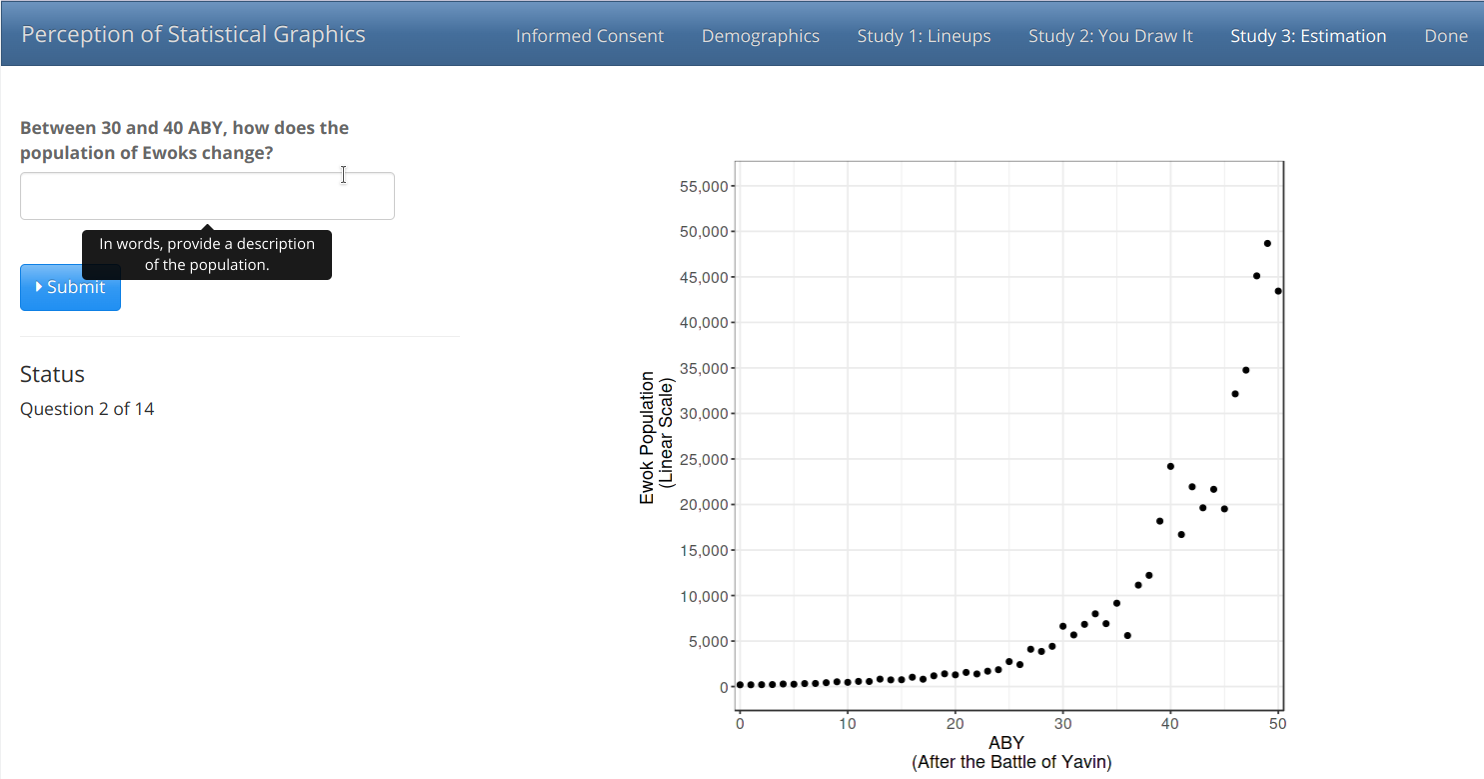
\includegraphics[keepaspectratio]{images/Estimation_describe_plot_crop.png}}

}

\caption{\label{fig-estimation-describe}This question asks users to
write out a description of how the population of Ewoks changes over
time, without any further cues, to determine whether participants
default to multiplicative or additive language descriptions.}

\end{figure}%

Of course, in an online, asynchronous experiment, every user interaction
with the testing materials (typically hosted on a web page) can also be
recorded along with time stamps, mouse positions, browser size and
screen resolution, and other information. While we have not used this
type of information heavily in our experimental analyses thus far, in
most experiments we collect time stamp data in order to assess how long
participants spend on each question. Typically, the first round of test
questions takes the longest for participants to complete. Additional
replicates do not usually affect accuracy (i.e.~there is no immediate
learning effect) until after `too many' tests cognitive fatigue proves
to be detrimental to accuracy (Chowdhury et al., 2018). This sweet spot
between replicates and fatigue depends on the cognitive burden in each
test and should factor into designing the experiment. In some
experiments, we have provided participants with supportive tools, such
as ``scratch pads'' and calculators built into the Shiny application to
support the complex calculations required to answer higher-level
numerical estimation questions (Figure~\ref{fig-estimation-calc}). In
order to be supportive, the tools must be easy to use, but assuming this
bar is met, the tools can reduce participant cognitive load while
recording a wealth of information. This information provides real
insight into how participants were looking at the data, what strategies
they tried and discarded for reading the chart, and what visual
estimation methods were used. While systematic analysis and modeling of
this data may be difficult, as it is usually messy and often must be
manually coded, the insights provided can be extremely useful. However,
unless participants are required to use these tools, it is difficult to
gather comprehensive information - those participants that don't use
supportive tools likely differ in meaningful ways from those who do. As
a result, the information gathered from supportive tools likely does not
generalize to the entire sample.

\begin{figure}

\centering{

\pandocbounded{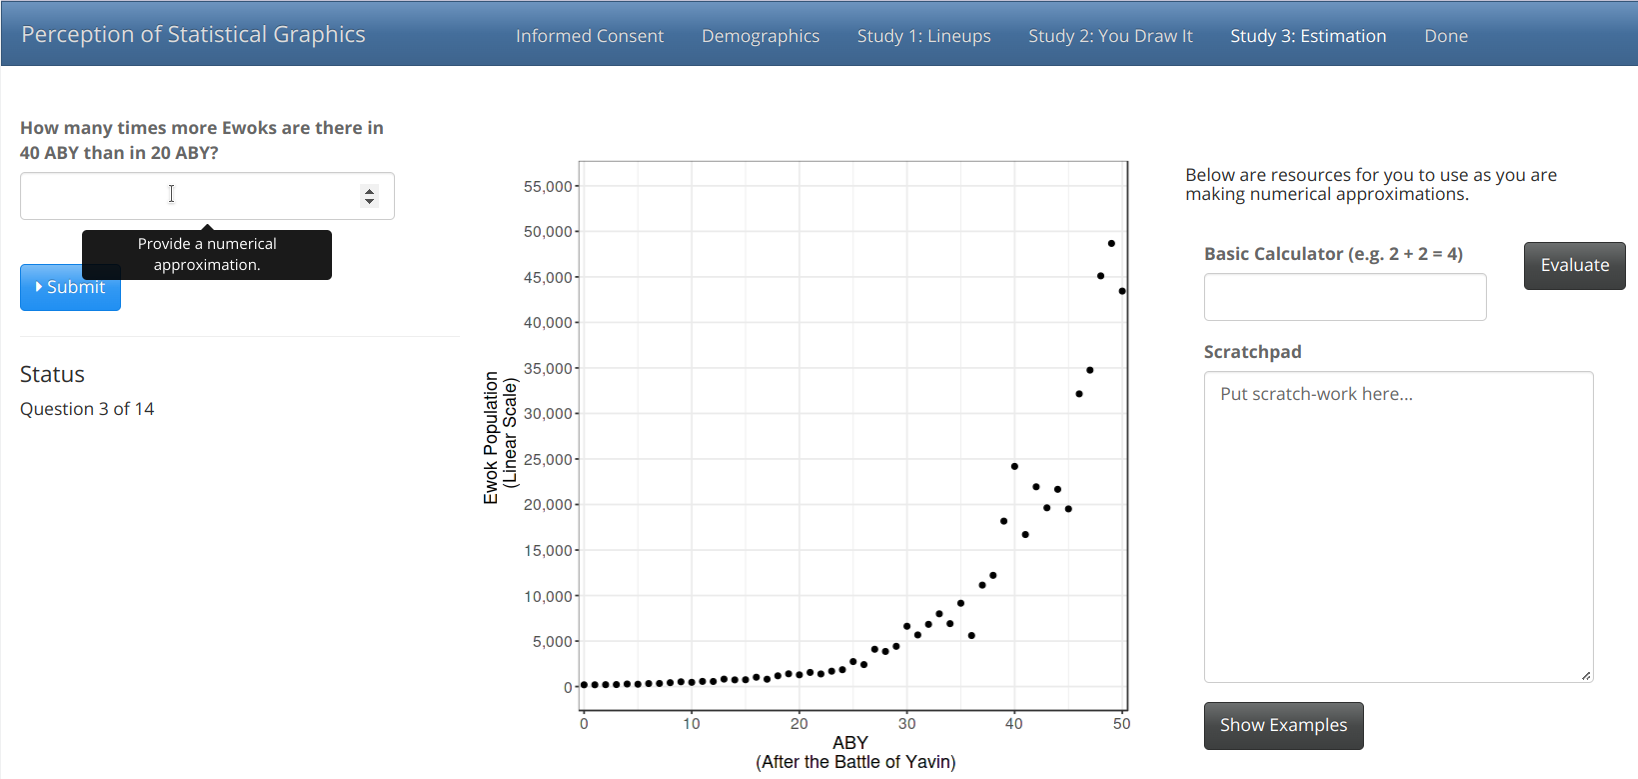
\includegraphics[keepaspectratio]{images/Estimation_numerical_screenshot_crop.png}}

}

\caption{\label{fig-estimation-calc}This question asks participants for
a numerical estimate, but provides a basic calculator and scratchpad.
All user interactions with the calculator and scratchpad are logged,
providing insight into the user's thought process and estimation
strategy.}

\end{figure}%

One of the most difficult components of designing an experiment which
asks users to directly estimate information from a chart using a full
scenario (background information, etc. as well as contextual details
from the chart) is that the questions must be extremely carefully
constructed. Mathematics education researchers provide guidelines for
selecting different levels of questioning in order to assess graph
comprehension: literal reading of the data, reading between the data,
and reading beyond the data (Curcio, 1987; Friel et al., 2001; Glazer,
2011; Wood, 1968). In a recent study, we identified questions based on
this framework to evaluate direct estimates and extend those estimates
to make comparisons between two points.

Even when great care is taken with the construction of the question,
participant answer accuracy is fundamentally limited by the fact that
many participants do not read and interpret the question with the care
and precision that it was written. Questions that ask participants to
e.g.~estimate the multiplicative change in a quantity at two time points
may be misunderstood as asking for an estimate of the additive
difference, and the resulting estimates are then one or more orders of
magnitude off of the correct answer. This is one area where lineup
methods are convenient - they do not depend on participants to
understand the nuances of language or scenarios built around the chart
under investigation. However, in some situations it may be sufficient to
ask participants to estimate direct numerical quantities that have
little contextual information, as done in (Vanderplas et al., 2019) when
assessing the accuracy of framed plots re-created from the Statistical
Atlas.

Another useful measurement strategy is to require participants to
\emph{engage directly} with an interactive visualization. This is useful
in a directed task, where users are asked to interact with the chart in
a specific way and the result is recorded, but it is also possible to
use interactive visualizations in an open-ended task, recording how
users engage with the graphic in an exploratory (as opposed to
goal-directed) manner. In one recent experiment, we asked participants
to forecast an exponential trend, with data presented on either a linear
or log scale. Using JavaScript code modified from New York Times
interactive graphics ``You Draw It'' features (Katz, 2017), we had users
draw trend lines with their computer mouse and make forecasts directly
on interactive charts, with the data and user-drawn predictions recorded
to our database (Robinson et al., 2023b). With interactive graphics
rendered using JavaScript (or other web libraries), the only limit to
the types of questions one can ask in testing graphics is one's ability
to write code to interact with the visualization library. This type of
testing method can be extremely natural for participants, but it also is
hard to generalize when discussing testing methods because of the
potential range of applications where it might be employed.

Whichever testing method is chosen should be appropriate to the type of
question under investigation and the level of visual and cognitive
engagement required to answer that question. While lineups are excellent
tools for assessing perceptual questions, they cannot address questions
aimed at understanding how people use charts within the wider context of
a story or practical task; this requires more direct methods with higher
ecological validity.

All of the testing methods described here require significant work to
develop a strategy for data generation appropriate for testing the
underlying question. For instance, when testing the perception of
exponential growth, we had to develop a model which would generate data
with varying growth rates, but where the data had a pre-specified domain
and range. If the null plots fail to capture the key visual
characteristics - such as trend, spread, or clustering - then any
standout visual differences may be attributed to those unintended
features, rather than the perceptual cue being tested. In other words,
if the nulls are too obviously different, participants might detect the
real plot for the wrong reason. Each testing method has specific
requirements, but it is important to carefully calibrate the model
parameters to allow for some variability, but not too much, and to
ensure that participants can succeed at the task and do not feel like
they are being made to analyze random noise. This Goldilocks-style
problem is the focus of the next section.

\section{Experiment Development Life
Cycle}\label{experiment-development-life-cycle}

Developing a graphics experiment is often a highly iterative process,
but it can help to approach the design process by first optimizing the
model and data generation method before spending time on optimizing the
specific stimuli or customizing the data collection platform. This is
important because the model parameters and data generation process
inform the experiment structure and thus impact decisions made
downstream.

Once the model and data generating mechanism are set, it is useful to
revisit the primary questions of interest and determine how to measure
the responses effectively. Secondary measures, such as response time,
free responses, and confidence level should also be determined. These
choices will inform the choice of a data collection platform and may
also inform the participant recruitment method.

Next, we recommend developing a preliminary data analysis plan,
specifying the general category of model which will be used
(e.g.~generalized linear mixed-effects model, t-test) and the contrasts
which are most interesting. This sets up the experimental design
decisions, but also ensures that as the data collection platform and
process is developed, any design constraints are considered. Development
of the data collection application is the next step, using draft
graphics and the set of participant response measures of interest.

There are at least 3 stages of testing in a graphics experiment:
informal tests, a pilot study, and the main experiment. The informal
tests are critical for identifying issues with the data collection
application, but can also be used to calibrate the number of tasks
required of each participant. As the number and complexity of tasks
increases, the number of trials we can ask participants to complete
during a session decreases. The informal testing stage allows
researchers to consider the tradeoffs inherent in the decision to reduce
the amount of information collected for each task, reduce the number of
tasks, or mitigate participant fatigue in other ways.

During preliminary testing, we use an optimistic number of trials per
participant, so that we can determine when participants become overly
fatigued. For instance, we might ask test participants to evaluate 20
graphical lineups (400 total plots), even though we expect to reduce the
number to 10 or 15 during the main experiment. We test the application
in individual or focus group sessions, often using graduate students,
colleagues, social media acquaintances, and conscripted family members.
After these participants complete the study, we ask questions about
fatigue to determine what range of trials per participant is reasonable.
At the end of our initial experiment tests, we have enough information
to determine the basic parameters of the experimental design (e.g.~how
many blocks in an incomplete block design can we have with the factors
under investigation). The number of trials a single participant can
complete without excessive fatigue impacts the number of blocks and the
strategy by which we allocate trials to each participant.

In addition, we must consider how long participants take to complete the
required number of trials. Completion time is used to determine
participant compensation (if using a participant recruiting platform).
Ethics boards and some recruitment platforms require that participants
are paid a reasonable wage for their time (currently, around \$15 US per
hour), and platforms may ask for median completion time and
automatically reject submissions from participants who are too far under
or over the specified time limits; they may also require additional
participant payments if the median time estimate is too far below the
actual average completion time during the experiment. Platforms may also
calculate fees based on both the participant payment and number of
participants recruited, with additional fees to recruit
e.g.~demographically representative samples; as a result, it can be
advantageous to balance cognitive load concerns with the fee structure
used by the selected recruitment platform.

The findings from the initial test of the experimental procedure are
then used to revise the data collection procedure in preparation for one
or more pilot studies. It is important to ensure that the software
platform, trial allocation, and other components of the experiment are
functioning as desired before a formal pilot study is conducted. In some
cases, the pilot study is as simple as a ``soft launch'' of the main
experiment, where the total number of trials is pre-specified and only a
few trials are released initially to ensure that data collection works
as expected. In others, the pilot study is conducted first, and results
from that study are used to determine the sample size for the main
experiment. At this point, data collection, analysis, and reporting
proceed much as in any other experiment.

\section{Developing a Model}\label{sec-model-dev}

Once the graphical task has been identified, it is necessary to develop
a model which can be used to explore the graphical features of interest
in a precise manner. This is the single longest part of the entire
experimental design and execution process, in part because choosing a
model that replicates important visual features of the data is extremely
complex (Cook et al., 2021; Hullman \& Gelman, 2021; Vanderplas, 2021).

There are two main options when developing a statistical model for
graphical testing: start with a large data set and sample from that data
set (Hofmann et al., 2012), or start from a model and sample data from
that model generating process (Robinson, 2022; Vanderplas \& Hofmann,
2015, 2017). This decision is largely determined by the availability of
a large data set containing the requisite features of interest and the
qualities being manipulated in the experiment. For instance, Hofmann et
al. (2012) used samples of different sizes from a pre-existing data set
to manipulate the amount of signal in each comparison; with a small
sample, there is less signal and the same amount of noise, making the
true plot harder to spot. In many situations, though, a convenient data
set with the right properties is harder to acquire, and it becomes
necessary to develop a sampling model to generate data for user
evaluation.

The tools we discuss in the remainder of this section can be applied
both to pre-existing data sets and to model-based sampling methods.

\subsection{Screening Parameters with
Simulation}\label{screening-parameters-with-simulation}

The choice of the parameter space used in testing is crucial to gain
insight from a study without putting too much burden on participants
with overlong studies. Choosing an appropriate space for testing
parameters is a well-known problem in psychometric testing: the space
considered should cover the area between `only some activation' to
`almost full activation' of an appropriate psychometric function (Schütt
et al., 2016; Valentin et al., 2024). When testing charts, visual
assessment is obviously key, but researchers can make use of statistical
indices related to the testing condition to narrow the parameter space
to a reasonable and efficient subset from which maximal information can
be acquired.\\
These statistical indices may also serve as quantitative proxies for the
difficulty of the visual task. To identify a statistical proxy for
visual difficulty that may help with narrowing the parameter space, it
can be useful to consider numerical measures used to estimate the same
types of visual information that will be assessed in the experiment. For
instance, we have used:

\begin{itemize}
\tightlist
\item
  \(R^2\) as a measure of the strength of a linear relationship,
\item
  Gini inequality as a measure of the strength of clustering, and
\item
  lack-of-fit statistics to assess the amount of curvature in an
  exponential relationship (shown in
  Figure~\ref{fig-lof-density-curves}).
\end{itemize}

Then, a wide range of potential combinations of parameter values or
sampling strategies can be explored and summarized graphically; if the
numerical statistic cannot differentiate between the null and target
under a condition, it is reasonable to think that a visual inspection of
the data may also not show significant results. As with any measure, it
is important that difficulty levels span a range from easy to hard; we
do not learn anything from finding out that everyone can distinguish all
of the combinations. This portion of the design is somewhat analogous to
selecting a range of doses of a chemical in a dose-response experiment.

\begin{figure}

\centering{

\pandocbounded{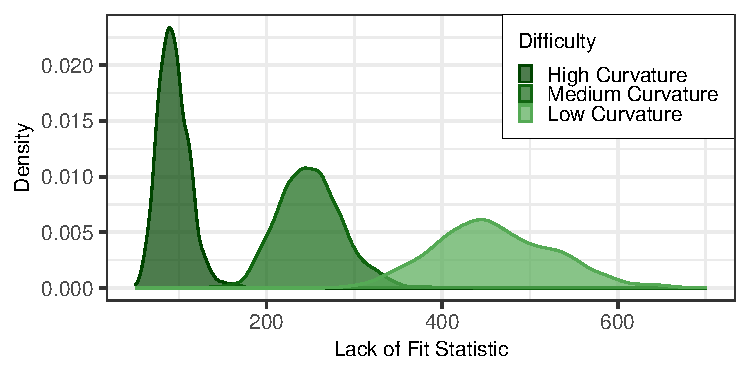
\includegraphics[keepaspectratio]{index-revised_files/figure-pdf/fig-lof-density-curves-1.pdf}}

}

\caption{\label{fig-lof-density-curves}Density plot of the lack of fit
statistic showing separation of selected difficulty levels: High
(obvious curvature), Medium (noticeable curvature), and Low (almost
linear). Each density plot is the result of 1000 simulations from a
model \(y_i = \alpha\cdot e^{\beta\cdot x_i + \epsilon_i} + \theta\),
where \(\epsilon \sim N(0, \sigma^2)\). \(\alpha\) and \(\theta\) were
selected after manipulation of \(\beta\) and \(\sigma\) to ensure that
all data generated had similar \(y\) ranges so as not to provide visual
cues about model differences outside of the plot curvature.}

\end{figure}%

While this method is certainly more critical for model-based sampling
methods, it is also important when data are generated by sampling from a
larger data set. When sampling from a larger dataset, parameters are
more often sample size and stratification methods, but it is still
important to iteratively assess the data generating procedure through
simulation. Using numerical proxies for visual characteristics of data
displays such as curvature, linearity, scatter, dispersion can assist
with identifying optimal parameter settings to use across different
experimental conditions. Even with this strategy, it is still critical
to fine-tune the parameter choices with visual calibration and pilot
testing.

\subsection{Fine-Tuning Parameter
Choices}\label{fine-tuning-parameter-choices}

Once an appropriate set of parameters are identified using the numerical
screening method, it is important to calibrate these parameter
selections visually. No numerical statistic is a perfect measure of what
we actually see: at best, they are approximations of what we might
potentially see. We have found it to be useful to have one experimenter
calibrate the model parameters at a gross level, and then have another
experimenter narrow in on the parameters which are visually reasonable
within the selected range. Then, both examiners visually inspect a large
number of plots generated using those parameters to get a sense for how
difficult the task at hand is (this strategy is also described by Lu et
al. (2022)). At some point, all experimenters become so visually
saturated with the nuances of the data generating mechanism that it may
become necessary to ``sanity check'' the protocol with family members,
friends, and colleagues. These informal focus groups provide extremely
useful feedback and can help to counteract the visual saturation of
being immersed in the design of a visualization experiment for months at
a time.

\subsection{Visual Assessment is
Critical}\label{visual-assessment-is-critical}

We cannot overstate the importance of visual assessment of your model
stimuli, preferably with fresh eyes. We highly recommend performing
several rounds of think-aloud pilot testing (e.g., focus groups) before
deploying an experiment. In support of this assessment, we offer up a
cautionary tale of our own experience: that of Vanderplas \& Hofmann
(2017), where we designed an experiment to test which plot aesthetics
promoted discovery of linear trends and/or clusters.

The experiment was a 2x3x3 factorial exploration of three data
generating parameters, with 3 replicates at each parameter combination
(54 data sets) and 10 aesthetic combinations (for a total of 540
lineups). Each lineup had 20 different sub-panels, so we should have
carefully visually inspected some 10,800 different panels. As is evident
from the fact that we're telling this story as a cautionary tale, we
missed a critical problem with our data-generating mechanism: when
clusters were assigned to randomly generated data after the fact, we
didn't control the cluster size, leading to clusters of one or two
points in relatively few sub-panels. This became particularly noticeable
when bounding ellipses were added to the plot, as the method used to
generate those ellipses required at least 3 points in the cluster. The
missing boundary ellipse in the corresponding sub-panels escaped our
notice during the stimuli proof-reading phase of the experiment, but did
not escape the notice of our participants, who only needed to examine
about 10 lineups each (around 200 panels). An example of one of the
problematic lineups is shown in Figure~\ref{fig-lineup-problems}: many
participants selected panel 16 because of the missing ellipse; not a
wrong choice, but certainly not the effect we intended to test.

\begin{figure}

\centering{

\pandocbounded{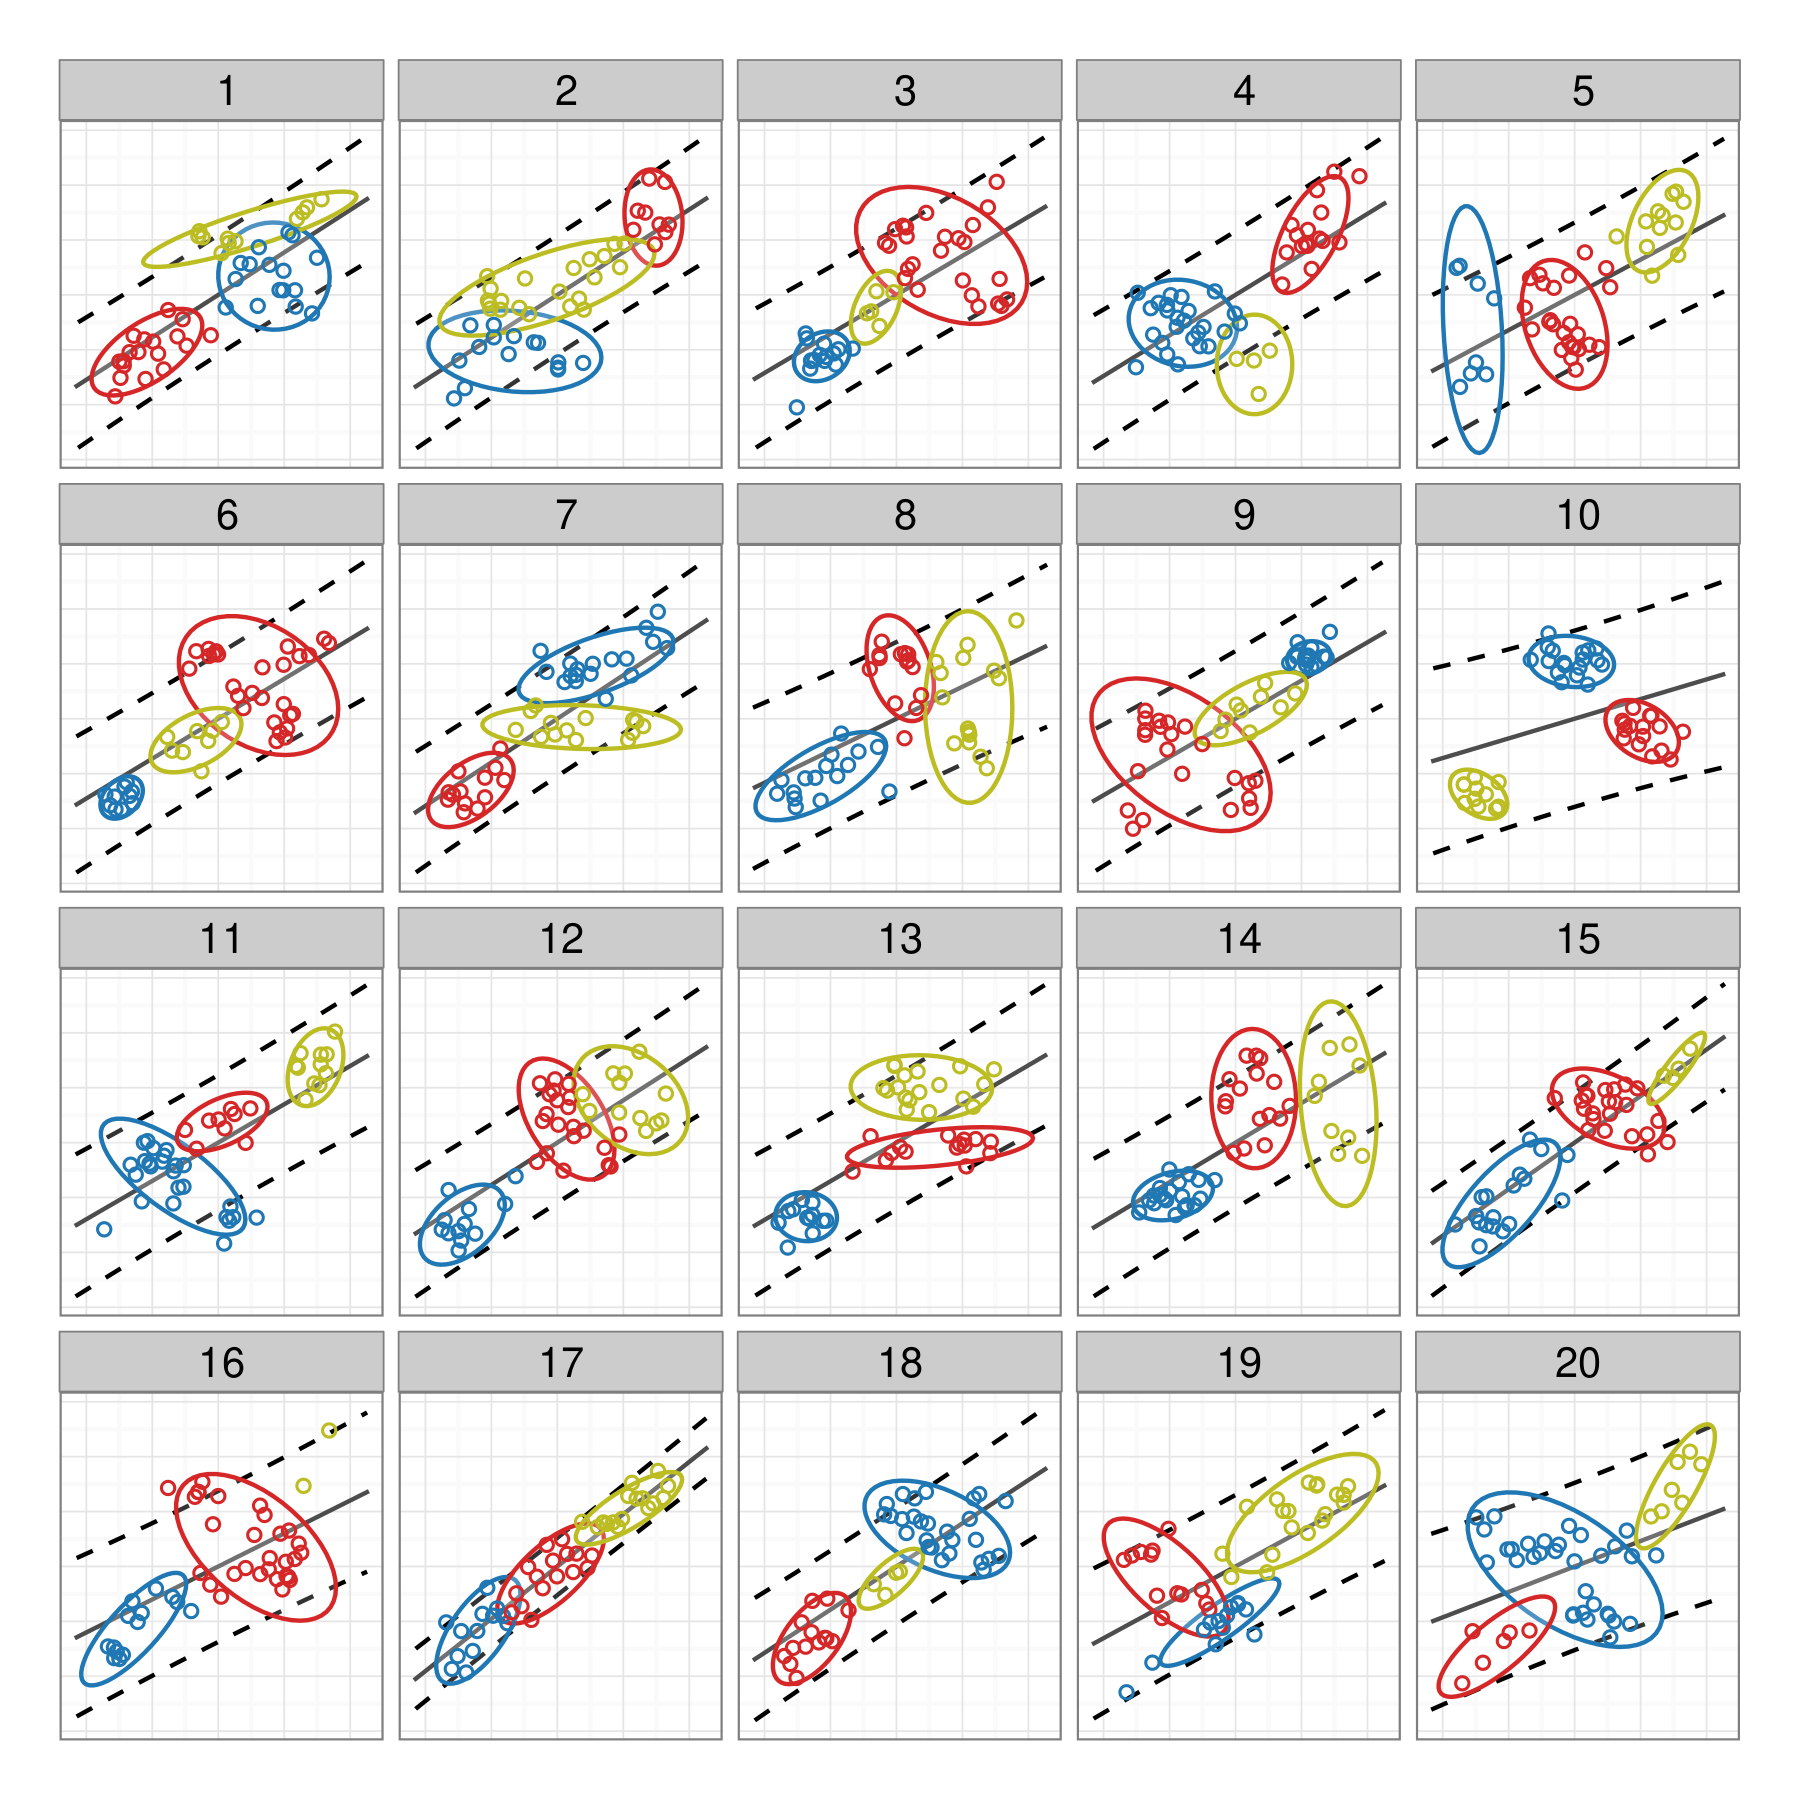
\includegraphics[keepaspectratio]{images/lineup-missing-ellipse.png}}

}

\caption{\label{fig-lineup-problems}A lineup from Vanderplas \& Hofmann
(2017). Panel 10 shows the clustered target data and panel 17 shows the
target data with a strong linear relationship; either of these target
panels was the expected choice. Unfortunately, panel 16 has only two
bounding ellipses shown, which is an unintentional difference that
resulted from a faulty method for assigning clusters to null plots; many
participants selected this panel instead of one of the target panels.}

\end{figure}%

One reason why it is so difficult to generate sampling models for visual
explorations is that our visual system is optimized for identifying
differences between groups. This ability can interfere with the natural
to use the null sampling models that might be used in equivalent
numerical tests when running experiments that use visualizations. We
re-ran the experiment using a different clustering method that
controlled the number of points in each group. Instead of noticing the
number of ellipses, participants instead used the differences in size
and shape of the ellipses formed when clustering after the data
generating procedure. That is, participants could still detect the
artificial nature of the induced clusters using other features. While it
can be difficult to get the data generating method right, it is
essential to conducting visual experiments that generalize well beyond
the effects shown in a single data set or phenomenon. This is also why
it is critical to include independent replications of the simulated
parameters, so that the results reflect variability due to the data
generation process, not just the specifics of a single simulated
dataset. The time and effort invested in this step at the outset of the
experiment pays dividends when it allows for clear generalization of the
experimental results to an entire statistical concept rather than a
single data set.

\section{Protocol Development}\label{sec-exp-dev}

It would be difficult to develop a full data generating model without
some idea of the experimental protocol: the basic equipment required for
the experiment, some idea of what questions users will answer, where and
how data will be collecteed, and so on. These experimental design
factors are fairly natural for scientists to accumulate over the course
of imagining and planning an experiment. When conducting graphical
tests, however, there are additional considerations beyond those taught
in a standard experimental design course. Experimenters must carefully
consider how much information participants should have about the
experiment, what platform to use to recruit participants, and the
experimental infrastructure underlying data collection. In addition to
our brief overview of considerations in our research, Kochari (2019) has
many helpful suggestions for conducting web-based cognitive and
perceptual studies that also apply to statistical graphics experiments.

Of course, more standard statistical design considerations, like
blocking, randomization, sample size, and analysis methodology are also
important; we will discuss these briefly in
Section~\ref{sec-exp-design}. Here, we focus primarily on the experiment
development process, with critical decisions in a roughly temporal
order.

\subsection{Infrastructure}\label{infrastructure}

We have conducted visualization experiments using a wide variety of
tools: custom web servers running interactive, PHP-based forms, generic
web survey platforms (Qualtrics, Google Forms) for static graphics, and
Shiny applications that control every part of the experiment interface
(instructions, generating completion codes for participant payment,
rendering interactive graphics, and generating fully randomized data for
each participant). In our research, Shiny has provided the right balance
between control over the experimental setting, procedure, etc. and the
intricate details of web server administration and management, however,
this balance is likely different for every lab and potentially for every
experiment.

When using Shiny to collect data, we store participant response data and
experiment parameters using SQLite tables, which are automatically
synchronized with cloud storage and tracked with version control. This
ensures that we have incremental records of the tables during data
collection, and that all data is stored across multiple locations,
guarding against hardware failures. In some studies, generated data is
unique to each participant; in these cases, we highly recommend saving
all generated data to a database as well, so that it is possible to go
back and examine responses alongside the data used to generate the
graphical stimuli. Hard drive space is extremely cheap relative to
almost any other cost in an experiment; saving all of the data is a
sensible measure.

\subsection{Participant Recruitment}\label{participant-recruitment}

There are several different, commonly used methods for recruiting
participants for visualization experiments and cognitive experiments
more broadly. The selection of participant recruitment method depends on
the infrastructure which will be used in the experiment, but the choice
of participant pool may be more critical to the experiment results than
the infrastructure and modality (Uittenhove et al., 2023).

We have used each of the following strategies in experiments:

\begin{itemize}
\item
  Validated, representative panels of participants offered by
  specialized polling groups. In the US, this includes
  \href{https://amerispeak.norc.org/us/en/amerispeak/about-amerispeak/panel-design.html}{NORC's
  AmeriSpeak} and
  \href{https://www.gallup.com/analytics/318911/us-social-research.aspx}{Gallup
  Panels}
\item
  Recruitment platforms designed for crowdsourcing research tasks,
  including \href{https://www.mturk.com/}{Amazon Mechanical Turk} and
  \href{https://www.prolific.com/}{Prolific}. Researchers may be able to
  obtain representative samples measured against census data along
  variables such as race, age, and sex, but participants are often more
  technologically sophisticated and educated than the general population
  on these platforms.
\item
  In-person studies. In person participants are commonly recruited from
  undergraduate students, but in some experiments it may be preferable
  to recruit participants from the local community. Students are often
  convenient for academic studies, as participation in experiments is
  often a component of introductory course experiential learning
  activities, as in Vanderplas et al. (2024). While the data generated
  from required classroom experiments may have higher variability, and
  it may be hard to generalize findings beyond undergraduate students,
  these studies can be conducted much more cheaply than studies
  conducted through online platforms or panels. Recruiting participants
  from the community for in-person research is also viable, but can be
  much more complicated, however, some topics, including research
  involving persons with specific disabilities, the elderly, or
  subject-matter experts may require recruiting participants outside the
  university.
\item
  Social media and email-based recruitment. Researchers may post
  directly to social media sites such as Twitter/X, Mastodon, and
  BlueSky, forums and discussion sites such as Reddit, or general email
  lists that may be purchased from universities and other marketing
  organizations. If the goal is to recruit a specific population, such
  as meterologists or forensic examiners, forums and email lists may be
  an extremely effective way to recruit participants. We have used the
  \href{https://web.archive.org/web/20250228110244/https://www.reddit.com/r/SampleSize/}{SampleSize
  subreddit} successfully and obtained participants that, while younger
  and more highly educated than those recruited from a platform, had
  similar results on visual estimation tasks (Vanderplas et al., 2019).
  When using samples obtained from acquaintances, researchers should try
  to obtain more diversity than was present in historical papers, such
  as Cleveland \& McGill (1984), where the authors sampled their
  colleagues (and their wives).
\end{itemize}

Rice et al. (2024) recruited participants using nationally
representative panel samples and found that conclusions from fully
representative samples of the population can be very different from
volunteer samples recruited using other services, as many people are
unmotivated to engage with charts, don't know how to read charts, or
impose pre-formed conclusions onto visual displays. While using
representative panel sampling products offered by organizations such as
NORC or Gallup is more expensive than samples from Amazon MTurk or
Prolific, these results may imply that results from less representative
participant recruitment methods may not generalize to the broader
population. People who participate in studies via online platforms are
more technologically sophisticated and educated than the general
population, and this bias may significantly impact the conclusions.
However, it is also reasonable to argue that higher education might make
someone more likely to use charts and data for decision-making.
Researchers designing a study should carefully consider whether the goal
of the study is to generalize results to the adult population or to a
subset of that population who make decisions based on data.

If data will be collected online, then we recommend considering the pros
and cons of panel-based sampling methods and online recruitment
platforms. While Amazon MTurk was once the only large platform for this
type of research (Heer \& Bostock, 2010), many researchers now prefer
Prolific because its participants appear to be more attentive to tasks
(Albert \& Smilek, 2023; Peer et al., 2022). Prolific's focus on
academic research rather than developing training data for machine
learning and AI means that its policies are tailored for these types of
projects and its users may be more interested in science than those on
other platforms. Experimenters should consider available options,
compare pricing structures (as these vary widely), and consider whether
add-on fees for e.g.~demographically representative samples are worth
the additional cost. It is also important to ensure that the platform
supports the type of user engagement required for the study. Online
recruitment platforms are more flexible than many panel survey platforms
and allow experimenters to use a much wider range of stimuli and
experimental designs, but this sacrifices some ability to generalize
results to a wider population.

\subsection{Participant Instructions}\label{participant-instructions}

It can be extremely helpful to include ``practice'' demonstrations of
the task to show the basic process, logic, and reasoning. While it is
tempting to make these tasks fully representative of the type of
judgement which will be required of participants, practice tasks which
are too close to the experimental task may bias participants. We have
found that it works well to have a relatively easy practice task which
utilizes a slightly different type of plot and/or type of data than what
will be tested in the experiment. In cases which require interactivity,
gif animations of the task being carried out are useful, as are
additional visual cues, such as the yellow box used in the `You Draw It'
task\footnote{See a gif of testing with `You Draw It'
  \href{https://i.imgur.com/GM5YSen.gif}{here}} to indicate that there
were points which were not completed. Demonstrations can reduce
cognitive load, but it is often critical not to prime participants to
focus on the specific effect manipulated during the experiment. Finding
the right examples and instructions to use in an experiment is a
delicate process: priming participants can reduce the generalizability
or relevance of the experiment, but if participants are confused about
what question to answer or how to complete the task, response
variability and participant cognitive load may be too high to detect an
effect. Pilot testing with a small group of volunteers who think aloud
while completing the experiment can be extremely helpful in identifying
problems with participant instructions. However, it is important that
some pilot participants have lower levels of mathematical and
statistical training that are similar to the participant population. One
technique that we have used is to wrap pilot testing into a presentation
about the experiment to a general audience, perhaps as part of an
undergraduate course or undergraduate research experience recruitment
activity. The experiential component increases participant understanding
of the research before the presenter explains the scientific goals
behind the project, and it is often easy to get feedback on the
experiment at the same time.

\subsection{Attention Checks and Answer
Validation}\label{attention-checks-and-answer-validation}

In a perfect world, all participants would be fully engaged in the
experiment, focusing only on that task from start to finish without
interruption or distraction. In this world, participants would
attentively read the unambiguous instructions for completing the
experiment and executing these instructions flawlessly. Unfortunately,
we do not live in this perfect world. Here, we focus primarily on
mechanisms which can be used to exclude data based on participant
noncompliance, rather than mechanisms which are used to automatically
withhold participant compensation.\\
There are several mechanisms that can be used to guard against or at
least identify participants who are not fully engaged in the experiment
or have severely misunderstood the instructions:

\begin{itemize}
\item
  Attention checks - questions inserted into the experiment which appear
  similarly to actual trials but which instruct participants to select a
  specific response or complete a trivial task (e.g.~select the result
  of 2+2). Participants who do not successfully complete a certain
  percentage of attention check tasks may be excluded from the
  experiment. More guidance on attention checks can be found in
  Muszyński (2023).
\item
  User input validation - mechanisms which reduce the potential
  parameter space of user inputs to a valid or reasonable set of
  parameters. Examples include not allowing participants to select
  negative variance values, requiring continuous user-drawn lines on an
  interactive chart, and even checking to ensure that the user's input
  is of the correct type. Validation mechanisms may also ensure that
  participants answer all questions before proceeding to the next page.
\item
  Time-based checks - Kochari (2019) suggests that in tasks with longer
  instructions, it may be useful to remove participants who did not
  spend a certain amount of time on the instructions page. Similarly, it
  may be justifiable to remove participants who completed the experiment
  in an unreasonably short or long amount of time. On the other end of
  the spectrum, participants who take several hours to complete an
  experiment with a median completion time of 15 minutes may have
  experienced technical issues or been distracted.
\end{itemize}

Pre-specifying conditions where participant data will be removed from
the study before analysis is critical for predictable issues, in order
to streamline the analysis and defend against p-hacking concerns. When
participants provide anomalous responses that are identified after the
experiment, it is much harder, but not impossible, to justify removing
the data. Justifications might include that no reasonable viewer would
have produced a certain response, as in Vanderplas \& Hofmann (2015), or
that the response most likely occurred due to a data entry error or a
fundamental misunderstanding of the question, but this is only viable if
the data is an egregious outlier. In less severe cases, it is often
preferable to leave the data in, increasing estimate variability but
avoiding the need to justify and defend data cleaning decisions.

\subsection{Demographic Data}\label{demographic-data}

It may be useful to ask a few more demographic questions about STEM
education level for studies which ask more of participants from a
mathematical standpoint; while lineup studies have not found strong
associations with those variables, lineup studies also do not require
participants to engage with the data presented in a chart in a way that
requires higher-order mathematical reasoning. This has allowed us to
make the argument to the ethics committee (institutional review board,
or IRB) that our research is exempt, as we do not collect enough
demographic information to identify participants, however, collecting
reduced demographic information occasionally comes at a cost. One recent
study examining the use of log scales and exponential data was conducted
using Prolific, which recruits participants from around the world; we
required only that participants were fluent in English to participate.
It was only after the experiment was completed that we realized that
different countries introduce logarithms as a concept at different
points during primary and secondary education; it might be that
individuals in some countries have much more experience with log scales
than those educated in the United States. We mention this only to point
out that while every experiment contains a few missed opportunities, it
is worth giving careful thought to the demographic questions asked of
participants and what information may be helpful during the analysis
stage.

\subsection{Ethics Review}\label{ethics-review}

Once the protocol is developed, researchers generally have enough
information to get approval from the ethics board to conduct an
experiment on human participants. We are most familiar with regulations
in the United States and can speak to that general process. Most
graphics experiments conducted in the US fall under the ``exempt''
category of experiments which require only basic review and approval.
These experiments record demographic information at a level that is not
individually identifiable, ask participants to complete tasks that
involve no risk, and experimenters record information which would not be
embarrassing to participants if exposed. In order to ensure that our
experiments fall into this category, we will often ensure that
demographic information and participant responses are collected and
stored separately from any identifiable information, such as e.g.~user
IDs from the participant recruitment platform that allow us to monitor
task completion and pay participants for their time. Researchers should
also ensure that they comply with privacy laws such as the European
\href{https://gdpr-info.eu/chapter-3/}{General Data Protection
Regulation (GDPR)}; complying with this law while collecting data which
is not identifiable can be complicated. We recommend consulting with
your ethics board and institutional recommendations in order to maintain
legal compliance and safeguard participant privacy.

\section{Experimental Design}\label{sec-exp-design}

In statistical design terms, most of our studies involve some type of
balanced incomplete block design, where participants are assigned to a
subset of experimental conditions which allow for estimation of the full
range of effects specified in the model. The particular structure of
these designs depends heavily on the factorial structure of the study
and the contrasts of interest. In some experiments, it is important that
participants see each set of data only once, while in others, it is
critical that participants see the same set of data represented
graphically under multiple conditions, at which point it becomes
necessary to manipulate the order of trials to ensure that participants
do not have back-to-back trials using the same data, because that might
influence the responses. When randomization and blocking are used in the
experiment, it is often beneficial to simulate the experiment before it
is conducted to ensure that the data collection platform is correctly
balancing and randomizing trials. Of particular concern is that in
online experiments with demographic controls, some categories fill
faster than others. In extreme circumstances, this can result in
imbalances in block allocation within subgroups, which may complicate
analysis of demographic data. It is preferable to iron out these issues
before the main study begins, rather than trying to patch the data
collection software in the middle of the study.

It is difficult to offer specific advice on the number of participants
to include in the study, because the experimental design, participant
engagement level, and the specific factors under investigation have such
a large effect on the number of trials one participant can reasonably
complete before fatigue effects increase response variance. The
cognitive fatigue constraints on the experimental design are important,
but otherwise, power calculations for graphics experiments are similar
to comparable experiments in other disciplines, in that a pilot study
provides the necessary inputs to the sample size calculation for the
main experiment. Some experts have begun to recommend that instead of
pilot-study informed power calculations, experimenters use a more
general approach based on the intended analysis method (Brysbaert,
2019). As power calculations for various statistical methods can be
easily found in any experimental design textbook (such as Easterling
(2015)), here we provide some basic guidelines based on past
experiments.

In psychophysical graphics experiments, such as Lu et al. (2022), there
are often fewer participants with many more trials per participant (28
participants, 250 trials each); the stimuli in these experiments are
often much simpler (e.g.~one or two plots instead of 20 in a lineup) and
engagement is limited to detection rather than estimation or prediction.
Psychophysics experiments, particularly those designed for analysis
using Rasch models, require that each participant assesses a full
factorial set of stimuli, whereas analysis with generalized linear mixed
models allows for use of incomplete blocks and other strategies that
spread the cognitive burden across several participants. These
experiments have also been traditionally completed in person, which may
also explain the large number of trials each participant is asked to
complete.

Online graphics experiments often have between 300 and 600 participants
(Robinson et al., 2025,), but this varies widely with the experimental
design, type of stimuli used, and level of participant engagement
required; Loy et al. (2016) and Vanderplas \& Hofmann (2017) had more
than 1300 participants, while Vanderplas \& Hofmann (2015) and
Vanderplas et al. (2019) had fewer than 150 participants. In-person
experiments (e.g. Vanderplas \& Hofmann, 2016) often use fewer
participants than online equivalents, but these experiments may require
more tasks of each participant, reflecting the increased logistical
costs of scheduling participants, supervising the experiment, and
entering the data, if tasks are completed on paper. In some cases,
in-person experiments may combat cognitive fatigue by scheduling the
experiment across multiple visits; this leaves experiments vulnerable to
participant drop-out effects, but can effectively balance cognitive load
and participant recruitment costs in some situations.

\section{Pilot Testing and Quality Assurance}\label{sec-pilot-test}

Once the data generating model is set, the protocol is developed, the
experiment is designed, and ethics paperwork has been submitted, the
next step is another round of testing. The goal of the initial sequence
of testing is to ensure that the experiment is set up properly and that
no issues have been overlooked. Pilot testing also provides an
opportunity to ensure that directions are clear, participants know what
they are supposed to be doing, and that the designed study has
sufficient power to detect an effect. Our studies usually go through 2-3
rounds of preliminary testing, with at least one of those rounds
involving any relatives and friends who are less technologically savvy.
We also purposely include talented individuals who can accidentally
crash any testing applications, as a way to harden our data collection
software before deployment.

One highly useful (but not strictly essential) component of an
experiment that can be set up during the pilot testing stage is a basic
analysis script which summarizes all data collected to date visually. We
have used such scripts in the past to produce automatically updating
dashboards or web pages, allowing for real time or near-real time
monitoring of data collection efforts. This provides an easy way to
summarize completion of the experiment so that individuals can receive
credit (if using services like MTurk or Prolific), but also allows
interested participants to see individual results, which can be a factor
when recruiting on social media. As data collection online can also
happen extremely quickly (300 participants in \textless2 hours in our
most recent Prolific experiment), this can improve data monitoring,
allowing any issues to be spotted and resolved quickly. If server load
is a potential issue, it may also help to release batches of trials over
a longer period of time in order to minimize the chance of having to
make participants wait for others to complete the task before the server
can handle additional connections\footnote{This is the one major
  drawback to our preferred solution of self-hosting a Shiny server to
  handle data collection: the free version of Shiny server is limited to
  about 15 connections at any given time. Prolific has recently added
  rate-limiting functions to the experimental control platform, which
  makes controlling the number of active jobs much easier.}. Batch trial
releases can also be used to ensure that participants are recruited
across different time zones; in some studies this is beneficial, while
in others it may be more important to control the release time to target
individuals in e.g.~North America rather than Europe.

\section{Analyzing the Data}\label{sec-analysis}

One constant with data analysis of these types of experiments is that no
matter how carefully the experiment is planned, designed, and executed,
there will be surprises. This is the dual curse and blessing of studying
human perception: the visual system never quite works the way that we
expect that it will, which provides endless fodder for science and
occasionally complicates the data analysis.

\subsection{Generalized Linear Mixed
Models}\label{generalized-linear-mixed-models}

The see-value approach (Chowdhury et al., 2020; Majumder et al., 2013;
Vanderplas et al., 2021) is extremely useful for single lineups, but
when a series of lineups that are part of a designed experiment are
used, generalized linear mixed models are a much simpler way to
summarize the overall effect of various manipulated factors (Hofmann et
al., 2012; Robinson et al., 2025; Vanderplas \& Hofmann, 2017). This
approach also works extremely well for psychometric experiments
(Vanderplas \& Hofmann, 2015), as psychometric models can be easily fit
into the framework of a generalized linear mixed model (Ju et al., 2024)
that has higher power than the Rasch models (Andrich, 1988; Lu et al.,
2022) which were historically recommended for these experiments. In
addition, similar model structures with different link functions can be
used to model accuracy, response time, and confidence, if all three
types of information are collected from participants during the
experiment.

\subsection{Numerical Estimation}\label{numerical-estimation}

There are additional considerations that should be expected when asking
participants to estimate numerical quantities. Anchoring and rounding
cause participant responses to cluster in ways that can bias statistical
estimators, requiring methods designed for these types of data (Heitjan
\& Rubin, 1991; Tourangeau et al., 2000; Ushakov \& Ushakov, 2017). An
alternative approach is to analyze the data graphically, as shown in
Figure~\ref{fig-density-rug}, which uses a density plot with rug
annotations to show individual participant point estimates. Rounding
effects can clearly be seen in the rug plot, but a kernel density
calculated using an appropriately selected bandwidth shows clear visual
differences between linear and log scale charts. In addition, a smaller
second mode can be seen in both linear and log conditions that
corresponds to the underlying model value; this suggests that a minority
of participants fit a mental regression model to the data and use that
model to estimate rather than estimating based off of the closest point.
When charts are carefully constructed to account for the experimental
structure and participant estimation strategies, displaying both
individual and aggregate responses, it is possible to demonstrate a
measurable difference between conditions without the need for
complicated statistical modeling which corrects for rounding and
anchoring effects.

While Figure~\ref{fig-density-rug} shows point estimates, the same
approach can be modified to account for experimental methods which
generate participant response curves. In these cases, rather than adding
a rug plot to a density plot showing aggregate estimates, it may be more
helpful to create spaghetti plots of individual estimates with a
superimposed consensus estimate and relevant annotations showing
e.g.~anchor points. The advantage of this approach is that it can
accommodate extremely messy data without requiring the extensive data
cleaning, modeling of heuristics like rounding and anchoring, and
elimination of nonsensical responses that might be necessary to fit a
statistical model. While statistical models are undoubtedly beneficial
in many situations, we have often found that graphical displays of
experimental results are at least as useful for analyzing and presenting
the results of graphical experiments.

\begin{figure}

\centering{

\pandocbounded{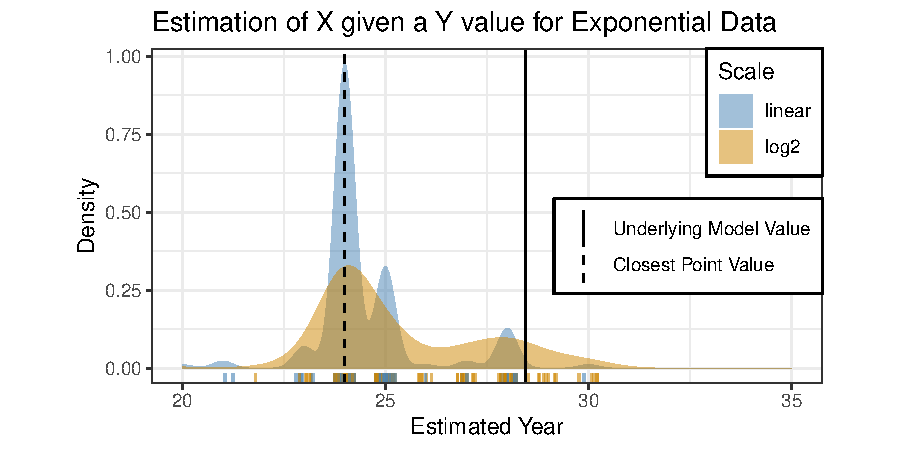
\includegraphics[keepaspectratio]{index-revised_files/figure-pdf/fig-density-rug-1.pdf}}

}

\caption{\label{fig-density-rug}Density of participant estimates for the
year (x-value) in which the population reaches 4000 (y-value). Colors
are associated to scale - linear (blue) and log (orange) - and vertical
lines indicate the true value based on the underlying model equation
(black solid) and closest point value based on the simulated data set
(black dashed). A jittered rug plot along the \(x\)-axis shows where
participant estimates were made. The plot shows anchoring occurred to
the closest point as shown by an increase in density around the dashed
line. Density peaks occurred at whole values indicating rounding
errors.}

\end{figure}%

\subsection{Direct Interactions}\label{direct-interactions}

If participants are making predictions and/or fitting visual statistics,
we have had success analyzing these responses by comparing the responses
to results from a statistical model to determine how visual statistics
differ from the numerical quantities derived mathematically. For
instance, in Robinson et al. (2023a), we calculate the deviation between
participant responses and the linear regression in `You Draw It'
experiments, then fitted generalized additive mixed models to summarize
the results across different experimental conditions to assess how
user-drawn predictions deviated from the statistical estimates. In other
direct interactions, it may be useful to compare participant selections
or annotations to closest points on the chart to assess anchoring
behavior; for discrete selections, methods discussed in numerical
estimation may also be useful.

\subsection{Qualitative Responses}\label{qualitative-responses}

In many cases, it is helpful to combine participants' qualitative
reasoning with their quantitative responses to designed graphical
experiments. This approach provides useful context as to what
participants use to make their decisions, and can be useful when
assessing why unexpected responses occurred. Qualitative questions can
be as simple as asking for a free response explanation of the
quantitative response(s), but it can also be effective to use
qualitative questions to prompt participants about problem solving
strategies, interesting features in the data, and more.

We have used word clouds to show overall themes in participant
explanations of why specific lineup panels were selected (Vanderplas \&
Hofmann, 2017); when paired with an appropriate linear model it became
clear that participants were fixating on unequal cluster size as a
visual cue. In cases where participants are provided with additional
utilities such as calculators and scratchpads, it can be useful to
select responses from individual participants which illustrate the
different types of calculations performed, but analyzing this data
quantitatively can be difficult, as it may be incomplete or difficult to
code systematically.

\section{Conclusion}\label{conclusion}

Testing features of visualization graphically using online platforms
provides an incredibly powerful and efficient way to establish empirical
guidelines for statistical graphics and visualization. There are nearly
endless ways to combine web graphics, user interactions, and data
collection to get insight into perception and use of graphics in
practical settings. We have been continually surprised at the richness
of the data collected in these experiments and the ability to combine
qualitative and quantitative assessment to support conclusions that are
both nuanced and of practical use when deciding how to design and
present data using visualizations.

In this paper, we have attempted to contextualize and motivate the logic
behind the process we use to design empirical graphics experiments.
We've discussed model development, experimental design considerations,
pilot testing, and data analysis methods that have been honed over many
successful and less-than-optimal experiments. While no experiment
involving humans ever goes exactly to plan, following this process helps
to avoid some of the most likely mishaps, ensuring that each new
experiment's ``bonus'' findings have only minimal impacts on the study's
overall utility.

While it can be difficult to conduct empirical tests of different
visualizations, the results of these experiments support guidelines for
graphical design and communication of statistical findings in an
accessible and explainable way. Many chart design guidelines and
recommendations are based on heuristics, but as scientists, we should
prefer guidelines which are based on empirical, experimentally derived
results over opinions. Testing statistical graphics and developing
empirically supported guidelines for chart creation promises to support
better scientific communication, which is critical for educating the
public about topics like climate change, public health, the risk of
severe weather and more.

\section{Author Statements}\label{author-statements}

\textbf{Conflict of Interest} The authors have no conflicts of interest
to declare in this manuscript.

\textbf{Funding} No outside funding was used to create this manuscript.

\textbf{Data Availability} This manuscript does not present any newly
collected data. Simulated data and code to create many of the images in
this paper can be found at
https://github.com/srvanderplas/Guide-Testing-Statistical-Graphics.

\section{References}\label{references}

\phantomsection\label{refs}
\begin{CSLReferences}{1}{0}
\bibitem[\citeproctext]{ref-albertComparingAttentionalDisengagement2023}
Albert, D. A., \& Smilek, D. (2023). Comparing attentional disengagement
between {Prolific} and {MTurk} samples. \emph{Scientific Reports},
\emph{13}(1), 20574. \url{https://doi.org/10.1038/s41598-023-46048-5}

\bibitem[\citeproctext]{ref-allenVisualizingScientificData2016}
Allen, E. A., \& Erhardt, E. B. (2016). Visualizing {Scientific} {Data}.
In J. T. Cacioppo, L. G. Tassinary, \& G. G. Berntson (Eds.),
\emph{Handbook of {Psychophysiology}} (4th ed., pp. 679--697). Cambridge
University Press. \url{https://doi.org/10.1017/9781107415782.031}

\bibitem[\citeproctext]{ref-andrichRaschModelsMeasurement1988}
Andrich, D. (1988). \emph{Rasch models for measurement} (1st ed.).
{SAGE} Publications.

\bibitem[\citeproctext]{ref-bertin1983semiology}
Bertin, J., \& Berg, W. J. (1983). \emph{Semiology of graphics:
Diagrams, networks, maps} (Vol. 1). University of Wisconsin press
Madison.

\bibitem[\citeproctext]{ref-d3}
Bostock, M., Ogievetsky, V., \& Heer, J. (2011). D3 {Data}-{Driven}
{Documents}. \emph{IEEE Transactions on Visualization and Computer
Graphics}, \emph{17}(12), 2301--2309. \url{https://doi.org/10/b7bhhf}

\bibitem[\citeproctext]{ref-brysbaertHowManyParticipants2019}
Brysbaert, M. (2019). How many participants do we have to include in
properly powered experiments? {A} tutorial of power analysis with
reference tables. \emph{Journal of Cognition}, \emph{2}(1).
\url{https://doi.org/10.5334/joc.72}

\bibitem[\citeproctext]{ref-bujaStatisticalInferenceExploratory2009}
Buja, A., Cook, D., Hofmann, H., Lawrence, M., Lee, E.-K., Swayne, D.
F., \& Wickham, H. (2009). Statistical inference for exploratory data
analysis and model diagnostics. \emph{Philosophical Transactions of the
Royal Society of London A: Mathematical, Physical and Engineering
Sciences}, \emph{367}(1906), 4361--4383.

\bibitem[\citeproctext]{ref-cairoFunctionalArtIntroduction2012}
Cairo, A. (2012). \emph{The {Functional} {Art}: {An} introduction to
information graphics and visualization}. New Riders.

\bibitem[\citeproctext]{ref-shiny}
Chang, W., Cheng, J., Allaire, J., Sievert, C., Schloerke, B., Xie, Y.,
Allen, J., McPherson, J., Dipert, A., \& Borges, B. (2021). \emph{Shiny:
Web application framework for r}.
\url{https://CRAN.R-project.org/package=shiny}

\bibitem[\citeproctext]{ref-chowdhury2018}
Chowdhury, N. R., Cook, D., Hofmann, H., \& Majumder, M. (2018).
Measuring Lineup Difficulty By Matching Distance Metrics With Subject
Choices in Crowd-Sourced Data. \emph{Journal of Computational and
Graphical Statistics}, \emph{27}(1), 132--145.
\url{https://doi.org/10.1080/10618600.2017.1356323}

\bibitem[\citeproctext]{ref-niladriroychowdhurySeeValueApp2020}
Chowdhury, N. R., Diehl, H., Broderick, T., \& Stein, A. (2020).
\emph{The {See} {Value} {App}: {Visual} {Decision} {Making} for {Drug}
{Development}}. https://rinpharma.com/publication/rinpharma\_183/.

\bibitem[\citeproctext]{ref-clevelandShapeParameterTwoVariable1988}
Cleveland, W. S., McGill, M. E., \& McGill, R. (1988). The {Shape}
{Parameter} of a {Two}-{Variable} {Graph}. \emph{Journal of the American
Statistical Association}, \emph{83}(402), 289--300.
\url{https://doi.org/10.1080/01621459.1988.10478598}

\bibitem[\citeproctext]{ref-clevelandGraphicalPerceptionTheory1984}
Cleveland, W. S., \& McGill, R. (1984). Graphical perception: {Theory},
experimentation, and application to the development of graphical
methods. \emph{Journal of the American Statistical Association},
\emph{79}(387), 531--554.
\url{https://doi.org/10.1080/01621459.1984.10478080}

\bibitem[\citeproctext]{ref-clevelandGraphicalPerceptionGraphical1985}
Cleveland, W. S., \& McGill, R. (1985). Graphical {Perception} and
{Graphical} {Methods} for {Analyzing} {Scientific} {Data}.
\emph{Science}, \emph{229}(4716), 828--833.
\url{https://doi.org/10.1126/science.229.4716.828}

\bibitem[\citeproctext]{ref-cookFoundationAvailableThinking2021}
Cook, D., Reid, N., \& Tanaka, E. (2021). The {Foundation} {Is}
{Available} for {Thinking} {About} {Data} {Visualization}
{Inferentially}. \emph{Harvard Data Science Review}, \emph{3}(3).
\url{https://doi.org/10.1162/99608f92.8453435d}

\bibitem[\citeproctext]{ref-croxtonGraphicComparisonsBars1932}
Croxton, F. E. (1932). Graphic {Comparisons} by {Bars}, {Squares},
{Circles}, and {Cubes}. \emph{Journal of the American Statistical
Association}, \emph{27}(177), 54--60.

\bibitem[\citeproctext]{ref-croxtonBarChartsCircle1927}
Croxton, F. E., \& Stryker, R. E. (1927). Bar {Charts} {Versus} {Circle}
{Diagrams}. \emph{Journal of the American Statistical Association},
\emph{22}(160), 473--482. \url{https://doi.org/10.2307/2276829}

\bibitem[\citeproctext]{ref-curcio1987comprehension}
Curcio, F. (1987). Comprehension of mathematical relationships expressed
in graphs. \emph{Journal for Research in Mathematics Education},
\emph{18}(5), 382--393.

\bibitem[\citeproctext]{ref-desnoyersTaxonomyVisualsScience2011}
Desnoyers, L. (2011). Toward a {Taxonomy} of {Visuals} in {Science}
{Communication}. \emph{Technical Communication}, \emph{58}(2), 16.

\bibitem[\citeproctext]{ref-dunbar1995scientists}
Dunbar, K. (1995). How scientists really reason: {Scientific} reasoning
in real-world laboratories. \emph{The Nature of Insight}, \emph{18},
365--395.

\bibitem[\citeproctext]{ref-easterlingFundamentalsStatisticalExperimental2015}
Easterling, R. G. (2015). \emph{Fundamentals of {Statistical
Experimental Design} and {Analysis}}. John Wiley \& Sons.

\bibitem[\citeproctext]{ref-eellsRelativeMeritsCircles1926}
Eells, W. C. (1926). The {Relative} {Merits} of {Circles} and {Bars} for
{Representing} {Component} {Parts}. \emph{Journal of the American
Statistical Association}, \emph{21}(154), 119--132.
\url{https://doi.org/10.2307/2277140}

\bibitem[\citeproctext]{ref-fewInformationDashboardDesign2006}
Few, S. (2006). \emph{Information {Dashboard} {Design}: {The}
{Effective} {Visual} {Communication} of {Data}}. O'Reilly Media,
Incorporated.

\bibitem[\citeproctext]{ref-friel2001making}
Friel, S., Curcio, F., \& Bright, G. (2001). Making sense of graphs:
Critical factors influencing comprehension and instructional
implications. \emph{Journal for Research in Mathematics Education},
\emph{32}(2), 124--158.

\bibitem[\citeproctext]{ref-glazer2011challenges}
Glazer, N. (2011). Challenges with graph interpretation: A review of the
literature. \emph{Studies in Science Education}, \emph{47}(2), 183--210.

\bibitem[\citeproctext]{ref-thinkaloud}
Haak, M., De Jong, M., \& Schellens, P. (2003). Retrospective vs.
Concurrent think-aloud protocols: Testing the usability of an online
library catalogue. \emph{Behaviour \& {Information Technology}},
\emph{22}, 339--351. \url{https://doi.org/10.1080/0044929031000}

\bibitem[\citeproctext]{ref-haemerDoubleScalesAre1948}
Haemer, K. W. (1948). Double {Scales} are {Dangerous}. \emph{The
American Statistician}, \emph{2}(3), 24--24.
\url{https://doi.org/10.1080/00031305.1948.10501588}

\bibitem[\citeproctext]{ref-haiderStrategiesDetectingDifference2021}
Haider, J. D., Pohl, M., Beecham, R., \& Dykes, J. (2021). Strategies
for detecting difference in map line-up tasks. In C. Ardito, R.
Lanzilotti, A. Malizia, H. Petrie, A. Piccinno, G. Desolda, \& K. Inkpen
(Eds.), \emph{Human-computer interaction - {INTERACT} 2021} (pp.
558--578). Springer International Publishing.
\url{https://doi.org/10.1007/978-3-030-85613-7_36}

\bibitem[\citeproctext]{ref-heerCrowdsourcingGraphicalPerception2010}
Heer, J., \& Bostock, M. (2010). Crowdsourcing graphical perception:
Using mechanical turk to assess visualization design. \emph{Proceedings
of the {SIGCHI} Conference on Human Factors in Computing Systems},
203--212. \url{https://doi.org/10.1145/1753326.1753357}

\bibitem[\citeproctext]{ref-heitjanIgnorabilityCoarseData1991}
Heitjan, D. F., \& Rubin, D. B. (1991). Ignorability and {Coarse}
{Data}. \emph{The Annals of Statistics}, \emph{19}(4), 2244--2253.
\url{https://doi.org/10.1214/aos/1176348396}

\bibitem[\citeproctext]{ref-power}
Hofmann, H., Follett, L., Majumder, M., \& Cook, D. (2012). Graphical
tests for power comparison of competing designs. \emph{IEEE Transactions
on Visualization and Computer Graphics}, \emph{18}(12), 2441--2448.
\url{https://doi.org/10/f4fwkz}

\bibitem[\citeproctext]{ref-vonhuhnFurtherStudiesGraphic1927}
Huhn, R. von. (1927). Further {Studies} in the {Graphic} {Use} of
{Circles} and {Bars}: {A} {Discussion} of the {Eell}'s {Experiment}.
\emph{Journal of the American Statistical Association}, \emph{22}(157),
31--39. \url{https://doi.org/10.2307/2277346}

\bibitem[\citeproctext]{ref-hullmanDesigningInteractiveExploratory2021}
Hullman, J., \& Gelman, A. (2021). Designing for {Interactive}
{Exploratory} {Data} {Analysis} {Requires} {Theories} of {Graphical}
{Inference}. \emph{Harvard Data Science Review}, \emph{3}(3).
\url{https://doi.org/10.1162/99608f92.3ab8a587}

\bibitem[\citeproctext]{ref-juOneModelThat2024}
Ju, W. (Will)., Vanderplas, S., \& Hofmann, H. (2024). One {Model} that
fits them {All}: {Psychometrics} with {Generalized Linear Mixed Effects
Models}. \emph{Electronic Imaging}, 1--9.
\url{https://doi.org/10.2352/EI.2023.35.1.VDA-A01}

\bibitem[\citeproctext]{ref-katzYouDrawIt2017}
Katz, J. (2017). You {Draw} {It}: {Just} {How} {Bad} {Is} the {Drug}
{Overdose} {Epidemic}? \emph{The New York Times}.
\url{https://www.nytimes.com/interactive/2017/04/14/upshot/drug-overdose-epidemic-you-draw-it.html}

\bibitem[\citeproctext]{ref-kirschenbaum2003comparative}
Kirschenbaum, S. S. (2003). Comparative {Cognitive} {Task} {Analysis}:
{The} {Cognition} of {Weather} {Forecasting}. \emph{Proceedings of the
{Human} {Factors} and {Ergonomics} {Society} {Annual} {Meeting}},
\emph{47}, 473--477. \url{https://doi.org/10.1177/154193120304700347}

\bibitem[\citeproctext]{ref-kochariConductingWebBasedExperiments2019}
Kochari, A. R. (2019). Conducting {Web-Based Experiments} for {Numerical
Cognition Research}. \emph{Journal of Cognition}, \emph{2}(1), 39.
\url{https://doi.org/10.5334/joc.85}

\bibitem[\citeproctext]{ref-kosslynGraphDesignEye2006}
Kosslyn, S. M. (2006). \emph{Graph {Design} for the {Eye} and {Mind}}.
Oxford University Press.

\bibitem[\citeproctext]{ref-kulhavyCartographicExperienceThinking1992}
Kulhavy, Pridemore, \& Stock. (1992). Cartographic experience and
thinking aloud about thematic maps. \emph{Cartographica}, \emph{29}(1),
1--9. \url{https://doi.org/10.3138/H61J-VX35-J6WW-8111}

\bibitem[\citeproctext]{ref-leeHowPeopleMake2016}
Lee, S., Kim, S.-H., Hung, Y.-H., Lam, H., Kang, Y.-A., \& Yi, J. S.
(2016). How do people make sense of unfamiliar visualizations?: A
grounded model of novice's information visualization sensemaking.
\emph{{IEEE} Transactions on Visualization and Computer Graphics},
\emph{22}(1), 499--508. \url{https://doi.org/10.1109/TVCG.2015.2467195}

\bibitem[\citeproctext]{ref-loyVariationsQQPlots2016}
Loy, A., Follett, L., \& Hofmann, H. (2016). Variations of {Q-Q Plots}:
{The Power} of {Our Eyes}! \emph{The American Statistician},
\emph{70}(2), 202--214.
\url{https://doi.org/10.1080/00031305.2015.1077728}

\bibitem[\citeproctext]{ref-loyDiagnosticToolsHierarchical2013}
Loy, A., \& Hofmann, H. (2013). Diagnostic tools for hierarchical linear
models. \emph{Wiley Interdisciplinary Reviews: Computational
Statistics}, \emph{5}(1), 48--61.
\url{https://doi.org/10.1002/wics.1238}

\bibitem[\citeproctext]{ref-luModelingJustNoticeable2022}
Lu, M., Lanir, J., Wang, C., Yao, Y., Zhang, W., Deussen, O., \& Huang,
H. (2022). Modeling just noticeable differences in charts. \emph{{IEEE}
Transactions on Visualization and Computer Graphics}, \emph{28}(1),
718--726. \url{https://doi.org/10.1109/TVCG.2021.3114874}

\bibitem[\citeproctext]{ref-majumderValidationVisualStatistical2013}
Majumder, M., Hofmann, H., \& Cook, D. (2013). Validation of visual
statistical inference, applied to linear models. \emph{Journal of the
American Statistical Association}, \emph{108}(503), 942--956.
\url{https://doi.org/10/f5gntt}

\bibitem[\citeproctext]{ref-muszynskiAttentionChecksHow2023}
Muszyński, M. (2023). Attention checks and how to use them: {Review} and
practical recommendations. \emph{Ask: Research and Methods},
\emph{32}(1), 3--38. \url{https://doi.org/10.18061/ask.v32i1.0001}

\bibitem[\citeproctext]{ref-peerDataQualityPlatforms2022}
Peer, E., Rothschild, D., Gordon, A., Evernden, Z., \& Damer, E. (2022).
Data quality of platforms and panels for online behavioral research.
\emph{Behavior Research Methods}, \emph{54}(4), 1643--1662.
\url{https://doi.org/10.3758/s13428-021-01694-3}

\bibitem[\citeproctext]{ref-asme-standards-graphics}
presentation, J. committee on standards for graphic. (1915). Preliminary
report published for the purpose of inviting suggestions for the benefit
of the committee. \emph{Publications of the American Statistical
Association}, \emph{14}(112), 790--797.
\url{http://www.jstor.org/stable/2965153}

\bibitem[\citeproctext]{ref-R}
R Core Team. (2022). \emph{R: A language and environment for statistical
computing}. R Foundation for Statistical Computing.
\url{https://www.R-project.org/}

\bibitem[\citeproctext]{ref-ribeccaSearchChartsData}
Ribecca, S. (2022). \emph{The data visualisation catalogue}.
https://datavizcatalogue.com.

\bibitem[\citeproctext]{ref-riceTestingPerceptualAccuracy2024}
Rice, K., Hofmann, H., du Toit, N., \& Mulrow, E. (2024). Testing
{Perceptual Accuracy} in a {U}.{S}. {General Population Survey Using
Stacked Bar Charts}. \emph{Journal of Data Science}, 1--18.
\url{https://doi.org/10.6339/24-JDS1121}

\bibitem[\citeproctext]{ref-emily-diss}
Robinson, E. A. (2022). \emph{Human {Perception} of {Exponentially}
{Increasing} {Data} {Displayed} on a {Log} {Scale} {Evaluated} {Through}
{Experimental} {Graphics} {Tasks}} {[}Doctoral, University of Nebraska,
Lincoln{]}.
\url{https://github.com/earobinson95/EmilyARobinson-UNL-dissertation/raw/main/EmilyRobinson-final-dissertation.pdf}

\bibitem[\citeproctext]{ref-robinson2023eye}
Robinson, E. A., Howard, R., \& VanderPlas, S. (2023a). Eye fitting
straight lines in the modern era. \emph{Journal of Computational and
Graphical Statistics}, \emph{32}(4), 1537--1544.

\bibitem[\citeproctext]{ref-robinson2023you}
Robinson, E. A., Howard, R., \& VanderPlas, S. (2023b). 'You draw it':
Implementation of visually fitted trends with r2d3. \emph{Journal of
Data Science}, \emph{21}(2), 281--294.

\bibitem[\citeproctext]{ref-robinsonPerceptionCognitiveImplications}
Robinson, E. A., Howard, R., \& Vanderplas, S. (2025). Perception and
{Cognitive Implications} of {Logarithmic Scales} for {Exponentially
Increasing Data}: {Perceptual Sensitivity Tested} with {Statistical
Lineups}. \emph{Journal of Computational and Graphical Statistics},
\emph{0}(ja), 1--14. \url{https://doi.org/10.1080/10618600.2025.2476097}

\bibitem[\citeproctext]{ref-schuttPainfreeAccurateBayesian2016}
Schütt, H. H., Harmeling, S., Macke, J. H., \& Wichmann, F. A. (2016).
Painfree and accurate bayesian estimation of psychometric functions for
(potentially) overdispersed data. \emph{Vision Research}, \emph{122},
105--123. \url{https://doi.org/10.1016/j.visres.2016.02.002}

\bibitem[\citeproctext]{ref-tourangeau_rips_rasinski_2000}
Tourangeau, R., Rips, L. J., \& Rasinski, K. (2000). \emph{The
psychology of survey response}. Cambridge University Press.
\url{https://doi.org/10.1017/CBO9780511819322}

\bibitem[\citeproctext]{ref-traftonTurningPicturesNumbers2000}
Trafton, G. J., Kirschenbaum, S. S., Tsui, T. L., Miyamoto, R. T.,
Ballas, J. A., \& Raymond, P. D. (2000). Turning pictures into numbers:
Extracting and generating information from complex visualizations.
\emph{International Journal of Human-Computer Studies}, \emph{53}(5),
827--850. \href{https://10.1006/ijhc.2000.0419}{10.1006/ijhc.2000.0419}

\bibitem[\citeproctext]{ref-tufte}
Tufte, E. (1991). \emph{The {Visual} {Display} of {Quantitative}
{Information}} (2nd ed.). Graphics Press.

\bibitem[\citeproctext]{ref-uittenhoveLabTestingWebTestingCognitive2023}
Uittenhove, D. K., Jeanneret, S., \& Vergauwe, E. (2023). From
{Lab-Testing} to {Web-Testing} in {Cognitive Research}: {Who You Test}
is {More Important} than how {You Test}. \emph{Journal of Cognition},
\emph{6}(1), 13. \url{https://doi.org/10.5334/joc.259}

\bibitem[\citeproctext]{ref-ushakovStatisticalAnalysisRounded2017}
Ushakov, N. G., \& Ushakov, V. G. (2017). Statistical analysis of
rounded data: {Recovering} of information lost due to rounding.
\emph{Journal of the Korean Statistical Society}, \emph{46}(3),
426--437. \url{https://doi.org/10.1016/j.jkss.2017.01.003}

\bibitem[\citeproctext]{ref-valentinDesigningOptimalBehavioral2024}
Valentin, S., Kleinegesse, S., Bramley, N. R., Seriés, P., Gutmann, M.
U., \& Lucas, C. G. (2024). Designing optimal behavioral experiments
using machine learning. \emph{{eLife}}, \emph{13}.
\url{https://doi.org/10.7554/eLife.86224}

\bibitem[\citeproctext]{ref-vanderplasDesigningGraphicsRequires2021}
Vanderplas, S. (2021). Designing {Graphics} {Requires} {Useful}
{Experimental} {Testing} {Frameworks} and {Graphics} {Derived} {From}
{Empirical} {Results}. \emph{Harvard Data Science Review}, \emph{3}(3).
\url{https://doi.org/10.1162/99608f92.7d099fd0}

\bibitem[\citeproctext]{ref-vanderplasEscapingFlatlandGraphics2024}
Vanderplas, S., Blankenship, E., \& Wiederich, T. (2024). Escaping
{Flatland}: {Graphics}, {Dimensionality}, and~{Human Perception}. In H.
Mori \& Y. Asahi (Eds.), \emph{Human {Interface} and the {Management} of
{Information}} (pp. 140--156). Springer Nature Switzerland.
\url{https://doi.org/10.1007/978-3-031-60114-9_11}

\bibitem[\citeproctext]{ref-vanderplasTestingStatisticalCharts2020}
Vanderplas, S., Cook, D., \& Hofmann, H. (2020). Testing {Statistical}
{Charts}: {What} {Makes} a {Good} {Graph}? \emph{Annual Review of
Statistics and Its Application}, \emph{7}(1).
\url{https://doi.org/10.1146/annurev-statistics-031219-041252}

\bibitem[\citeproctext]{ref-vanderplasFramedReproducingRevisiting2019}
Vanderplas, S., Goluch, R., \& Hofmann, H. (2019). Framed! {Reproducing}
and {Revisiting} 150 year old charts. \emph{Journal of Computational and
Graphical Statistics}.
\url{https://doi.org/10.1080/10618600.2018.1562937}

\bibitem[\citeproctext]{ref-sineillusion}
Vanderplas, S., \& Hofmann, H. (2015). Signs of the {Sine} {Illusion} --
{Why} {We} {Need} to {Care}. \emph{Journal of Computational and
Graphical Statistics}, \emph{24}(4), 1170--1190.
\url{https://doi.org/10.1080/10618600.2014.951547}

\bibitem[\citeproctext]{ref-vanderplasSpatialReasoningData2016}
Vanderplas, S., \& Hofmann, H. (2016). Spatial {Reasoning} and {Data
Displays}. \emph{IEEE Transactions on Visualization \& Computer
Graphics}, \emph{22}(1), 459--468.
\url{https://doi.org/10.1109/TVCG.2015.2469125}

\bibitem[\citeproctext]{ref-clusters}
Vanderplas, S., \& Hofmann, H. (2017). Clusters {Beat} {Trend}!?
{Testing} {Feature} {Hierarchy} in {Statistical} {Graphics}.
\emph{Journal of Computational and Graphical Statistics}, \emph{26}(2),
231--242. \url{https://doi.org/10.1080/10618600.2016.1209116}

\bibitem[\citeproctext]{ref-vanderplasStatisticalSignificanceCalculations2021}
Vanderplas, S., Röttger, C., Cook, D., \& Hofmann, H. (2021).
Statistical significance calculations for scenarios in visual inference.
\emph{Stat}, \emph{10}(1). \url{https://doi.org/10.1002/sta4.337}

\bibitem[\citeproctext]{ref-ggplot2}
Wickham, H. (2016). \emph{ggplot2: Elegant graphics for data analysis}.
Springer-Verlag New York. \url{https://ggplot2.tidyverse.org}

\bibitem[\citeproctext]{ref-wickhamGraphicalInferenceInfovis2010}
Wickham, H., Cook, D., Hofmann, H., \& Buja, A. (2010). Graphical
inference for infovis. \emph{IEEE Transactions on Visualization and
Computer Graphics}, \emph{16}(6), 973--979.
\url{https://doi.org/10.1109/TVCG.2010.161}

\bibitem[\citeproctext]{ref-wilkinsonGrammarGraphics1999}
Wilkinson, L. (1999). \emph{The grammar of graphics}. Springer.
\url{http://public.ebookcentral.proquest.com/choice/publicfullrecord.aspx?p=3085765}

\bibitem[\citeproctext]{ref-wood1968objectives}
Wood, R. (1968). Objectives in the teaching of mathematics.
\emph{Educational Research}, \emph{10}(2), 83--98.

\end{CSLReferences}




\end{document}
